\documentclass[10pt]{beamer}
%\mode<presentation>{}

\usepackage{media9}
\usepackage{amssymb,amsmath,amsthm,enumerate}
\usepackage[utf8]{inputenc}
\usepackage{array}
\usepackage[parfill]{parskip}
\usepackage{graphicx}
\usepackage{caption}
\usepackage{subcaption}
\usepackage{bm}
\usepackage{amsfonts,amscd}
\usepackage[]{units}
\usepackage{listings}
\usepackage{multicol}
\usepackage{multirow}
\usepackage{tcolorbox}
\usepackage{physics}
\newcommand{\R}{\mathbb{R}}
\usepackage{algorithm2e}
\usepackage{lastpage}
% Enable colored hyperlinks
\hypersetup{colorlinks=true}

% The following three lines are for crossmarks & checkmarks
\usepackage{pifont}% http://ctan.org/pkg/pifont
\newcommand{\cmark}{\ding{51}}%
\newcommand{\xmark}{\ding{55}}%

% Numbered captions of tables, pictures, etc.
\setbeamertemplate{caption}[numbered]

%\usepackage[superscript,biblabel]{cite}
\usepackage{algorithm2e}
\renewcommand{\thealgocf}{}

% Bibliography settings
\usepackage[style=ieee]{biblatex}
\setbeamertemplate{bibliography item}{\insertbiblabel}
\addbibresource{references.bib}

% Glossary entries
\usepackage[acronym]{glossaries}
\newacronym{ML}{ML}{machine learning}



\theoremstyle{remark}
\newtheorem*{remark}{Remark}
\theoremstyle{definition}

\newcommand{\empy}[1]{{\color{darkorange}\emph{#1}}}
\newcommand{\empr}[1]{{\color{blue}\emph{#1}}}
\newcommand{\examplebox}[2]{
\begin{tcolorbox}[colframe=darkcardinal,colback=boxgray,title=#1]
#2
\end{tcolorbox}}

\usetheme{Stanford} 
\def \i  {\item}
\def \ai {\item[] \quad \arrowbullet}
\newcommand \si[1]{\item[] \quad \bulletcolor{#1}}
\def \wi {\item[] \quad $\ \phantom{\Rightarrow}\ $}
\def \bi {\begin{itemize}\item}
\def \ei {\end{itemize}}
\def \be {\begin{equation*}}
\def \ee {\end{equation*}}
\def \bie {$\displaystyle{}
\def \eie {{\ }$}}
\def \bsie {\small$\displaystyle{}
\def \esie {{\ }$}\normalsize\selectfont}
\def \bse {\small\begin{equation*}}
\def \ese {\end{equation*}\normalsize}
\def \bfe {\footnotesize\begin{equation*}}
\def \efe {\end{equation*}\normalsize}
\renewcommand \le[1] {\\ \medskip \lefteqn{\hspace{1cm}#1} \medskip}
\def \bex {\begin{example}}
\def \eex {\end{example}}
\def \bfig {\begin{figure}}
\def \efig {\end{figure}}
\def \btheo {\begin{theorem}}
\def \etheo {\end{theorem}}
\def \bc {\begin{columns}}
\def \ec {\end{columns}}
\def \btab {\begin{tabbing}}
\def \etab {\end{tabbing}\svneg\svneg}
\newcommand \col[1]{\column{#1\linewidth}}
\def\vneg  {\vspace{-5mm}}
\def\lvneg {\vspace{-10mm}}
\def\svneg {\vspace{-2mm}}
\def\tvneg {\vspace{-1mm}}
\def\vpos  {\vspace{5mm}}
\def\lvpos {\vspace{10mm}}
\def\svpos {\vspace{2mm}}
\def\tvpos {\vspace{1mm}}
\def\hneg  {\hspace{-5mm}}
\def\lhneg {\hspace{-10mm}}
\def\shneg {\hspace{-2mm}}
\def\thneg {\hspace{-1mm}}
\def\hpos  {\hspace{5mm}}
\def\lhpos {\hspace{10mm}}
\def\shpos {\hspace{2mm}}

\logo{
\includegraphics[height=0.4in]{./style_files/kaust_academy_logo.png}}

% commands to relax beamer and subfig conflicts
% see here: https://tex.stackexchange.com/questions/426088/texlive-pretest-2018-beamer-and-subfig-collide
\makeatletter
\let\@@magyar@captionfix\relax
\makeatother

\title[Computer Vision]{Computer Vision}
%\subtitle{Subtitle Of Presentation}

%\beamertemplatenavigationsymbolsempty

\begin{document}

\author[KAUST Academy]{
	\begin{tabular}{c} 
	\Large
	Naeemullah Khan\\
    \footnotesize \href{mailto:naeemullah.khan@kaust.edu.sa}{naeemullah.khan@kaust.edu.sa}
\end{tabular}
\vspace{-4ex}}

\institute{
	\vskip 20pt
	\begin{figure}
		\centering
		\begin{subfigure}[t]{0.5\textwidth}
			\centering
			
\includegraphics[height=0.5in]{./style_files/kaust_logo.png}
		\end{subfigure}
% 		~ 
% 		\begin{subfigure}[t]{0.5\textwidth}
% 			\centering
% 			
\includegraphics[height=0.33in]{./style_files/kaust_academy_logo.png}
% 		\end{subfigure}
	\end{figure}
	\vskip 20pt
	KAUST Academy \\
	King Abdullah University of Science and Technology\\
	\vskip 3pt
}

% \date{June 15, 2020}
\date{\today}

\begin{noheadline}
\begin{frame}\maketitle\end{frame}
\end{noheadline}


\setbeamertemplate{itemize items}[default]
\setbeamertemplate{itemize subitem}[circle]

\begin{frame}{Table of Contents}
\begin{itemize}
    \item Data Handling
    \item Data Augmentation
    \item Transfer Learning
    \item Ensembling
    \item Dropout
    \item Batch Normalization
    \item Full Training Workflow
\end{itemize}
    
\end{frame}

\begin{frame}{Learning Outcomes}
\begin{itemize}
    \item Implement efficient data handling techniques using PyTorch's Dataset and DataLoader classes
    \item Apply appropriate data augmentation strategies based on error analysis
    \item Utilize transfer learning effectively for different scenarios and dataset sizes
    \item Understand ensemble methods to improve model performance
    \item Apply regularization techniques like Dropout and Batch Normalization
    \item Design a complete deep learning training workflow from initial setup to infrence
\end{itemize}
\end{frame}



\begin{frame}{Practical Deep Learning}
\begin{itemize}
    \item Practical Implementation of Deep Learning algorithms is just as much an art as it is a science.
    \item The main takeaways if not to start from scratch rather to build on top of the previous knowledge.
    \item Today, we will look at some important tools used in the practical implementation of Deep Learning algorithms.

\end{itemize}
    
\end{frame}



\begin{frame}[allowframebreaks]{DataLoaders}
\begin{itemize}
    \item As we have previously established that Deep Learning has been made possible by large amount of data and computational resourse
    \item An important aspect to keep in mind is the data handling:
    \begin{itemize}
        \item How do we handle large amounts of data?
        \item How to we read different components of data (from possible different parts of our hard drive) and provide it to our training algorithms?
        \item How do we feed this data to SGD algorthims in a streamlined manner?
    \end{itemize}

    \item PyTorch provides Dataset and DataLoaders to handle data in an efficient manner.
    \item We will extend the Dataset and DataLoaders class to construct our own Dataloaders


    
\end{itemize}
\framebreak

\begin{itemize}
    \item Datasets in PyTorch: The \texttt{torch.utils.data.Dataset} class is an abstract base class used to define and manage datasets for training and evaluation.
    \item Custom Dataset Creation: You can create a custom dataset by subclassing \texttt{Dataset} and implementing 
    \begin{itemize}
        \item  \texttt{\_\_len\_\_()} (returns dataset size) and 
        \item \texttt{\_\_getitem\_\_()} (fetches a single data sample).
    \end{itemize}
    
    \item DataLoaders for Batching: \texttt{torch.utils.data.DataLoader} is used to load data in mini-batches, shuffle data, and utilize multiprocessing for efficiency.
    \item Built-in Datasets: PyTorch provides datasets in \texttt{torchvision.datasets} and \texttt{torchtext.datasets}, making it easy to load common datasets like MNIST, CIFAR-10, and IMDB.
\
\end{itemize}

    
\framebreak

    \begin{figure}
    \centering
    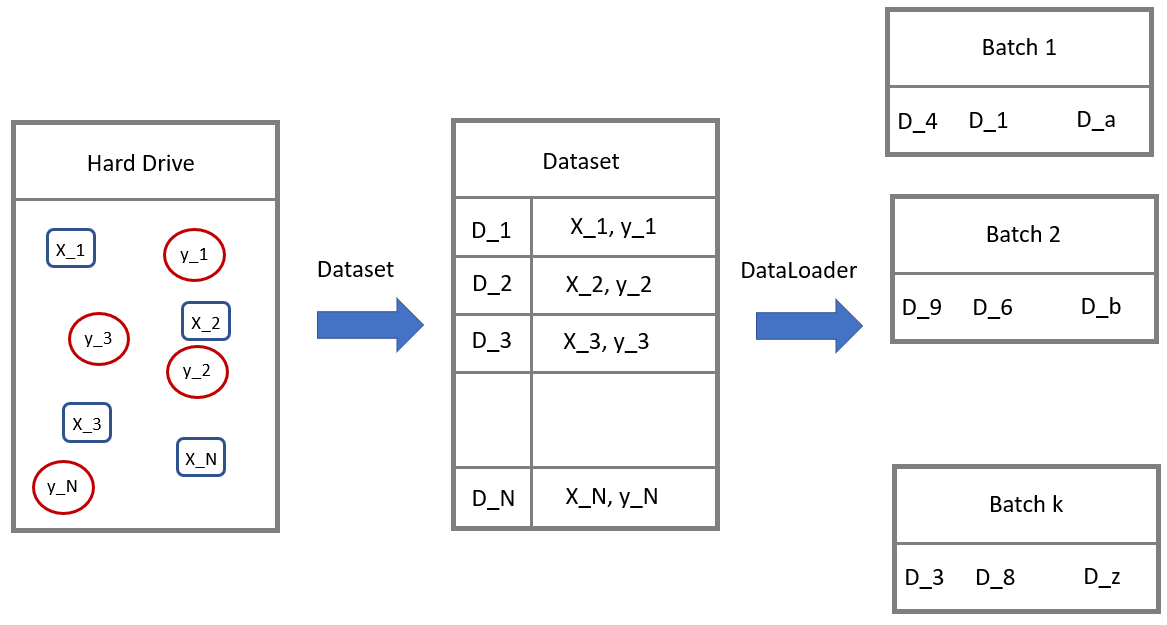
\includegraphics[width=1.0\textwidth,height=1.0\textheight,keepaspectratio]{./images/dataloaders.png}
    \end{figure}
\end{frame}

\begin{frame}[allowframebreaks]{Data Augmentation}
\begin{itemize}
    \item Data is the fundamental building block of any machine learning algorithm
    \item In several applications we don’t have access to unlimited data
    \item So we use Data Augmentation techniques to improve the preformance of our models
    \item Note: It is better to spend time on data rather than fine-scale architecture search in deep learning

\end{itemize}

\framebreak

\begin{itemize}
    \item Create virtual training samples
    \begin{itemize}
        \item Horizontal flip
        \item Random crop
        \item Color casting
        \item Geometric distortion
        \item Translation
        \item Rotation
    \end{itemize}

\end{itemize}

\framebreak
    \begin{figure}
    \centering
    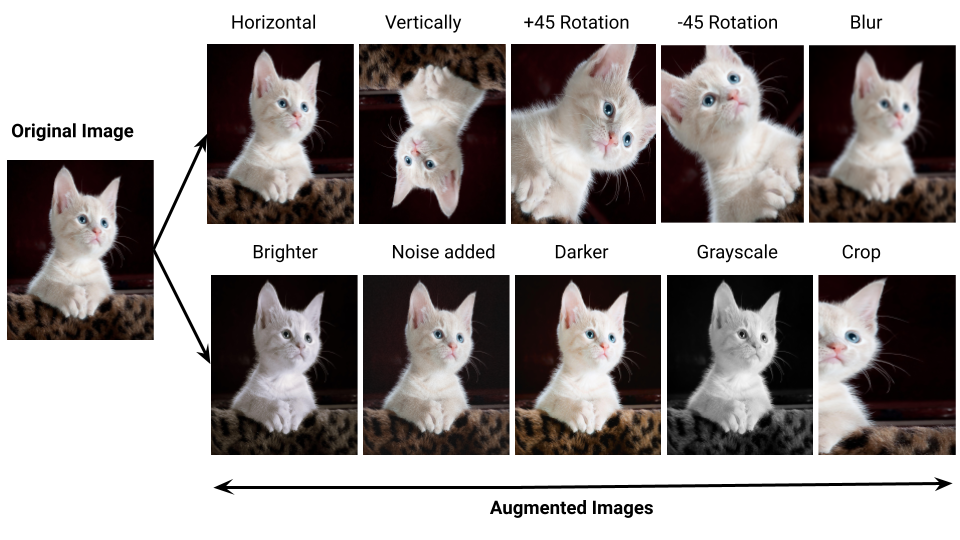
\includegraphics[width=1.0\textwidth,height=1.0\textheight,keepaspectratio]{./images/data_augmentation.png}
    \end{figure}
\footnotetext{ \url{https://pranjal-ostwal.medium.com/data-augmentation-for-computer-vision-b88b818b6010}}
\end{frame}

\begin{frame}[allowframebreaks]{Data Augmentation (cont.)}

    \begin{figure}
    \centering
    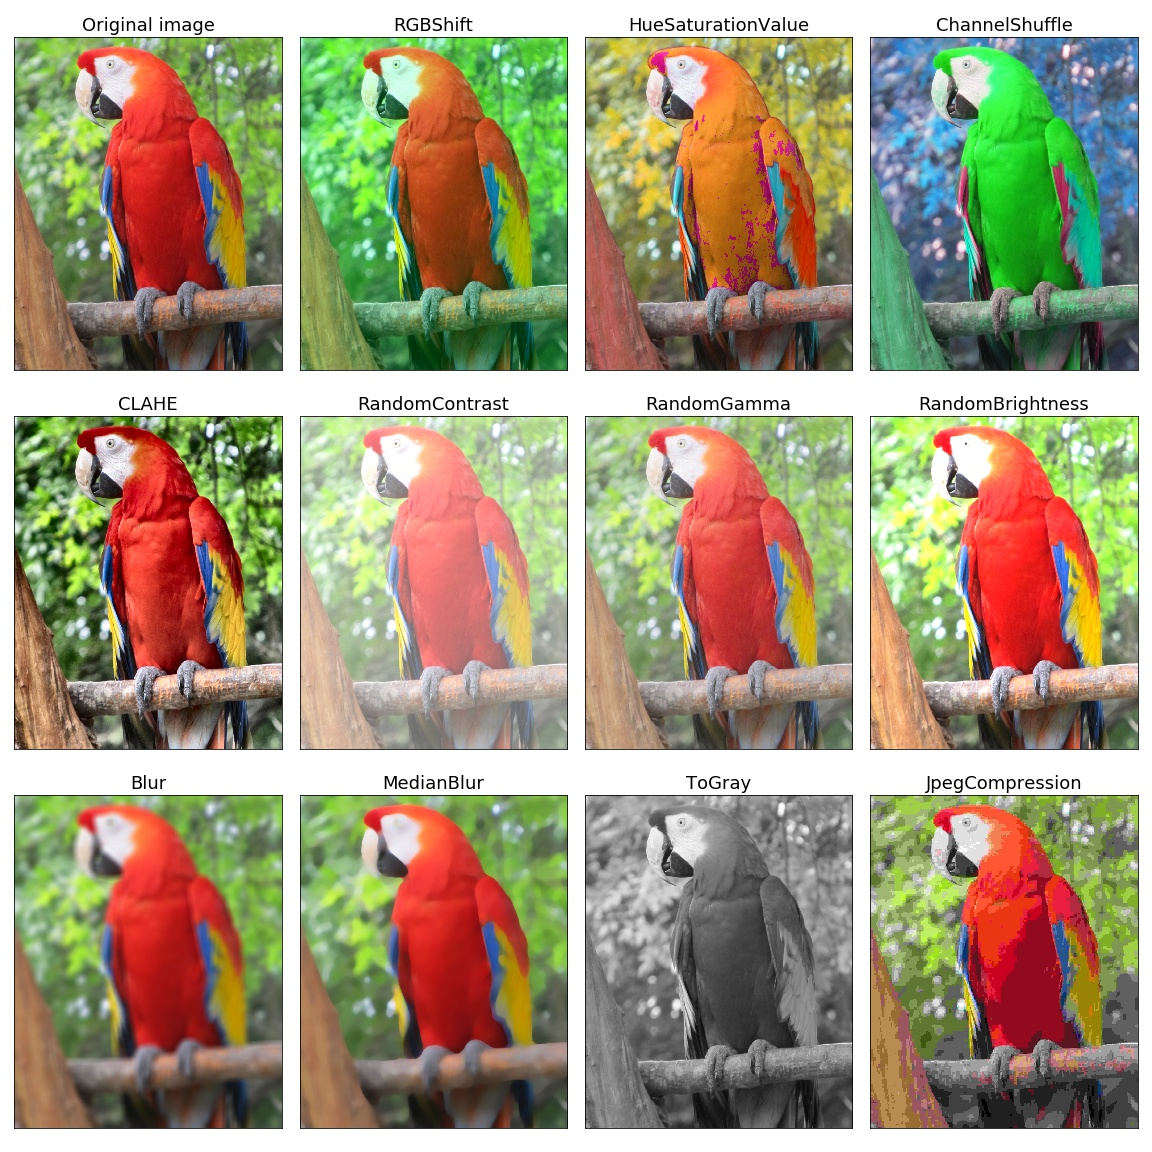
\includegraphics[width=.8\textwidth,height=.8\textheight,keepaspectratio]{./images/augmentation_new.jpg}
    \end{figure}
\footnotetext{To simplify data augmentation, tools like  \url{https://github.com/albumentations-team/albumentations}}

\end{frame}

\begin{frame}{Data Augmentation (cont.)}
\begin{itemize}
    \item But, there are many types of augmentations. How do we choose the right ones for our task?

\end{itemize}

\end{frame}

\begin{frame}{Data Augmentation (cont.)}
\begin{itemize}
    \item But, there are many types of augmentations. How do we choose the right ones for our task
    \item \textbf{Answer: Error Analysis} – Identify model weaknesses and apply augmentations that address those issues.
\end{itemize}
\end{frame}

\begin{frame}{Error Analysis for Data Augmentation}
\begin{itemize}
    \item \textbf{Steps:}
    \begin{enumerate}
        \item Train a baseline model.
        \item Make predictions on validation data.
        \item Inspect the worst predictions to identify model weaknesses.
        \item Apply relevant augmentations to address these issues.
    \end{enumerate}

    \item \textbf{Examples:}
    \begin{itemize}
        \item \textbf{Failure with small objects} → Use \textit{Scale Augmentation}.
        \item \textbf{Failure with different colors/environments} → Use \textit{Color Augmentations}.
        \item \textbf{Failure with rotated images} → Use \textit{Rotation Augmentations}.
        \item \textbf{Failure with blurry images} → Use \textit{Noise Augmentations}.
        \item \dots etc.
    \end{itemize}
\end{itemize}
\end{frame}



\begin{frame}{Data Augmentation}
\begin{itemize}
    \item \textbf{Note}: Data augmentation is applied only to the training data.
    \item Applying it to validation/test data \textbf{directly} would lead to \textbf{incorrect evaluation and misleading performance metrics}.
\end{itemize}
\end{frame}

\begin{frame}{Data Augmentation}
\begin{itemize}

       \item However, there is a special inference technique called \textbf{Test-Time Augmentation (TTA)} where multiple augmented versions of the same image are passed through the model separately, and the predictions are averaged to improve accuracy.




\end{itemize}
\begin{figure}
    \centering
    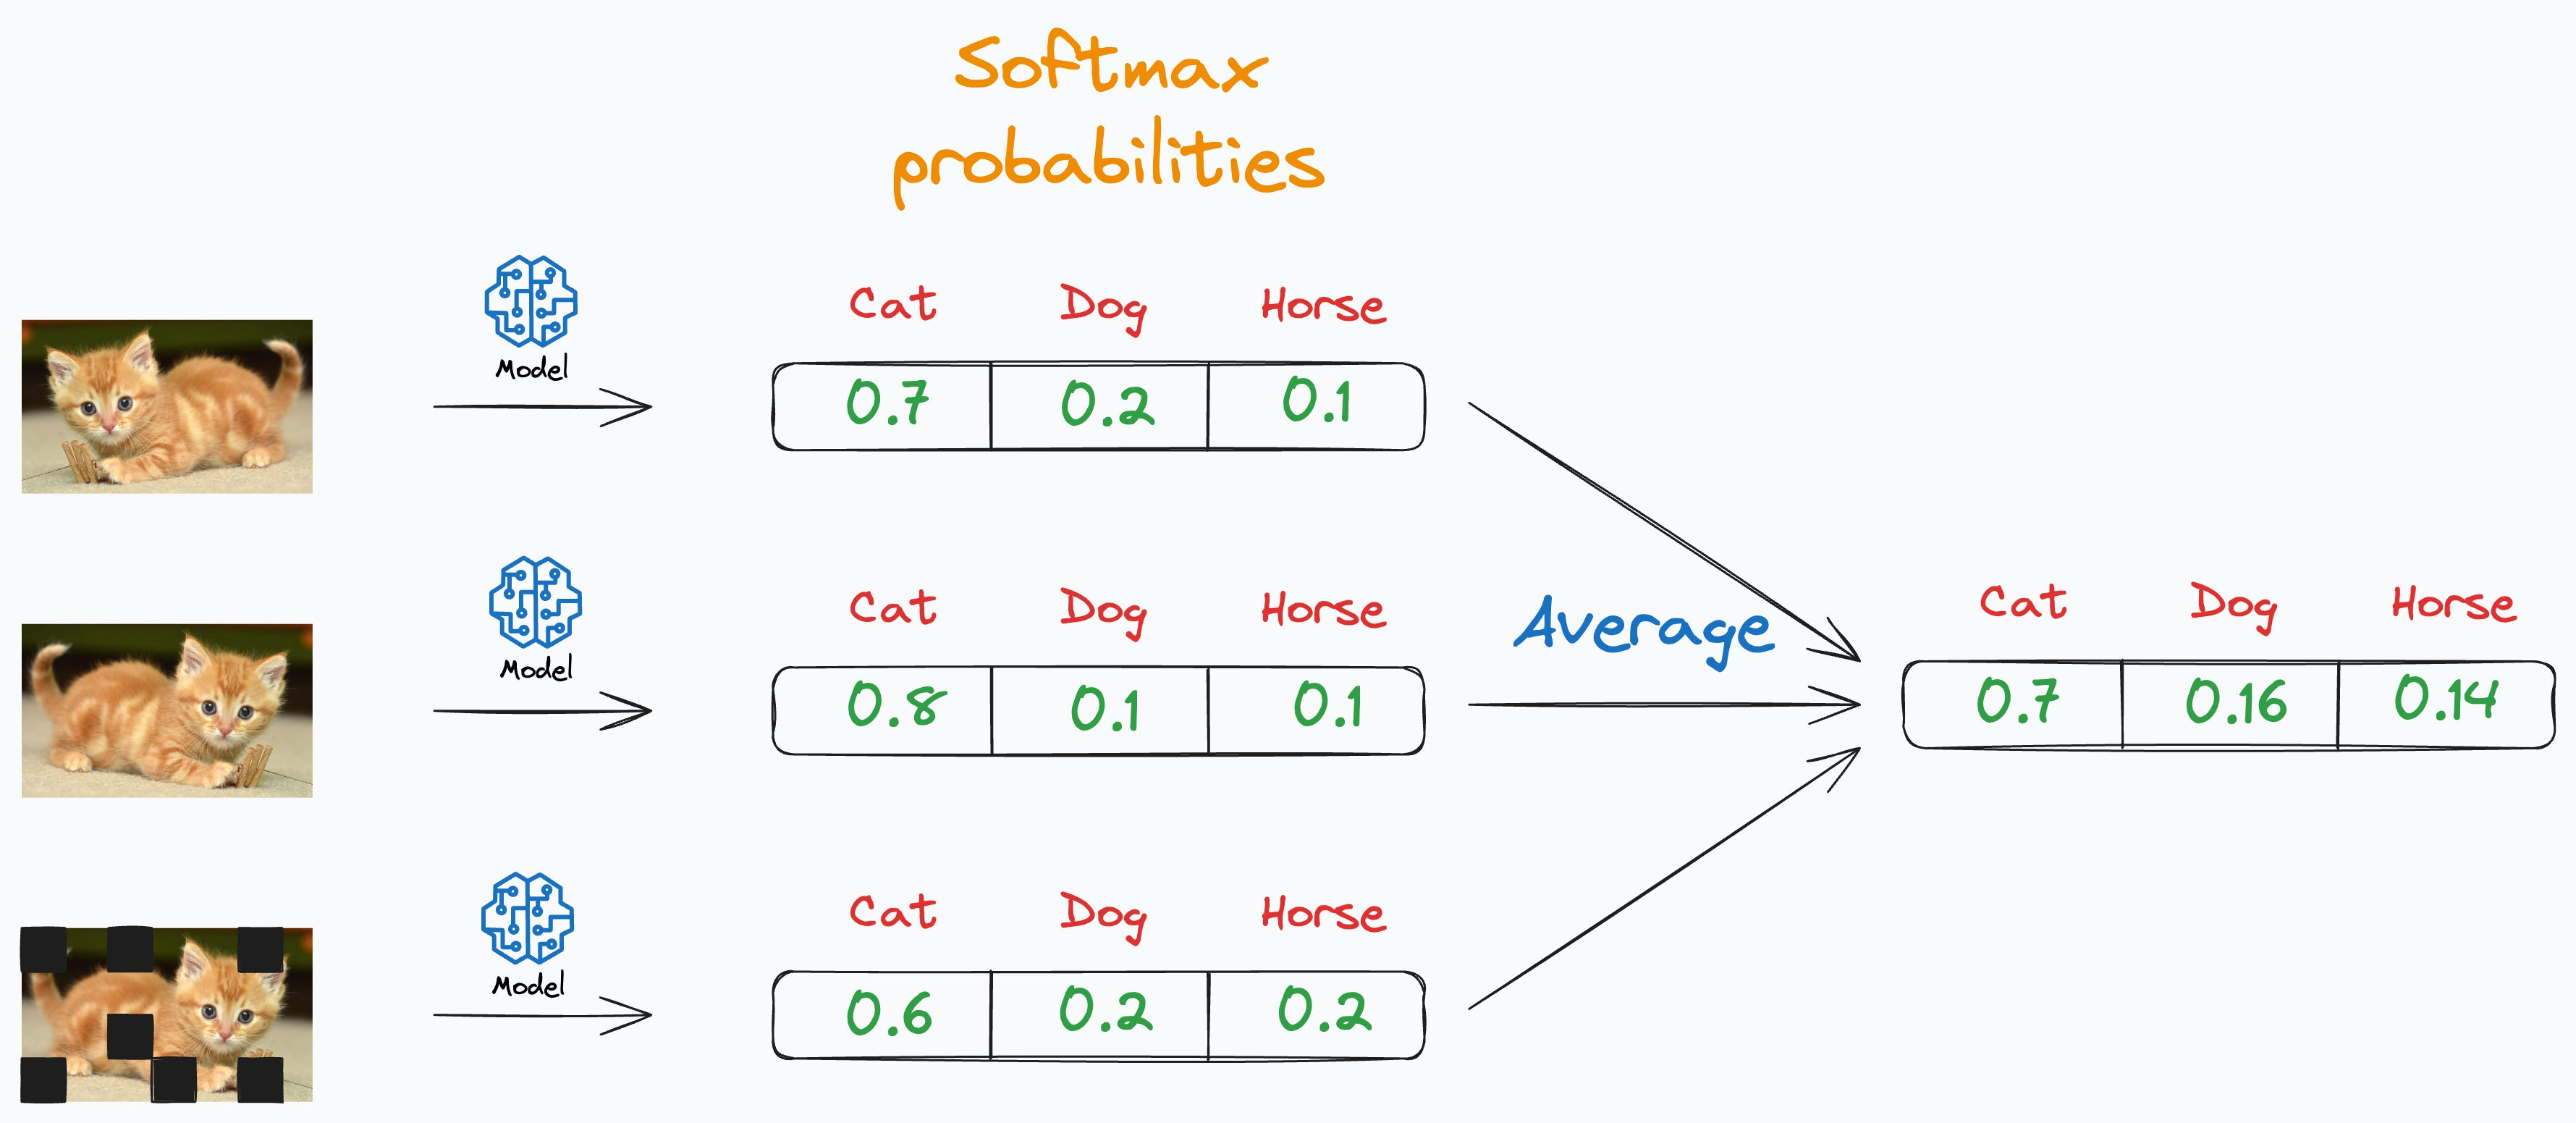
\includegraphics[width=1.0\textwidth,height=1.0\textheight,keepaspectratio]{./images/tta.jpg}
    \caption{Test-time Augmentation}
    \end{figure}

\end{frame}

\begin{frame}{Data Augmentation}
\begin{itemize}

    \item TTA is an advanced technique.

    \item Applying it requires \textbf{custom scripts} to generate augmented versions of test images, pass them through the model, and aggregate predictions.


\end{itemize}
\end{frame}




\begin{frame}[allowframebreaks]{Transfer Learning}
\begin{itemize}
    \item \textbf{What is Fine-Tuning?}  
    \begin{itemize}
        \item A strategy in \textbf{transfer learning} where a pre-trained model is adapted to a new task.
        \item Instead of training from scratch, we start from a model already trained on a related task.
    \end{itemize}
    \item \textbf{Why use Fine-Tuning?}  
    \begin{itemize}
        \item Saves time and computational resources.
        \item Improves performance, especially with limited data.
    \end{itemize}
\end{itemize}
\end{frame}


\begin{frame}[allowframebreaks]{When to fine-tune your model?}
    \begin{itemize}
        \item New dataset is small + similar distribution to original dataset:
        \begin{itemize}
            \item Freeze (or partially freeze) feature extraction layers and fine-tune the classifier.
        \end{itemize}

        \item New dataset is small + different distribution to original dataset:
        \begin{itemize}
            \item Use the pretrained network as a generic feature extractor and train a light classifier on top (e.g., SVM).
            \item In modern practice, you might also freeze earlier layers and selectively fine-tune later layers.
        \end{itemize}
        \item New dataset is large, regardless of the original data distribution:
        \begin{itemize}
            \item Fine-tune the entire network (both features extractor and classifier).
        \end{itemize}
    \end{itemize}
\end{frame}



\begin{frame}{Finetuning}
    \begin{figure}
    \centering
    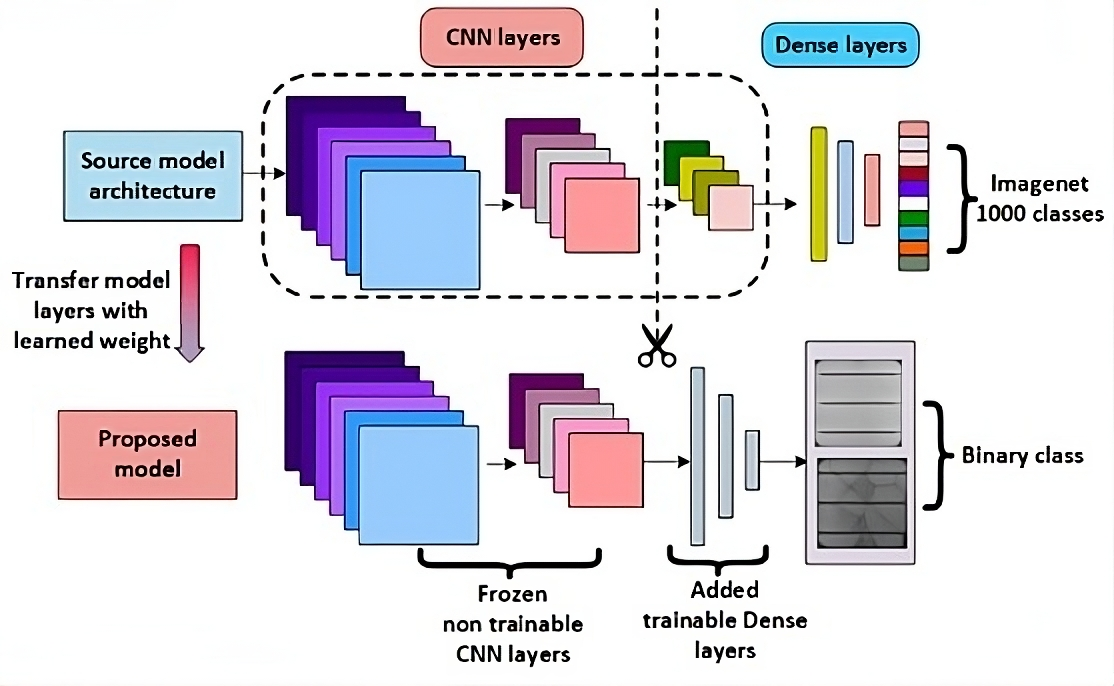
\includegraphics[width=1.0\textwidth,height=1.0\textheight,keepaspectratio]{./images/Finetuning_fig.png}
    \caption{Learning and Transferring Mid-Level Image Representations using Convolutional Neural Networks }
    \end{figure}

\end{frame}

\begin{frame}{Ensembling}
\begin{itemize}
    \item No single model is perfect. Different models make different types of errors.
    \item Let’s visualize the predictions of two different models:
\end{itemize}

\begin{figure}
    \centering
    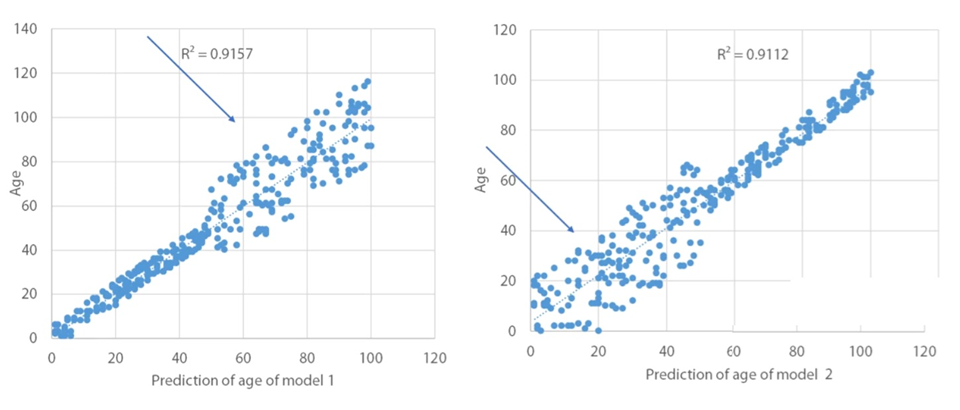
\includegraphics[width=1.0\linewidth]{./images/ensembling1.png} 
    \caption{Predictions of Model 1 and Model 2}
\end{figure}
\end{frame}

\begin{frame}{Ensembling}
\begin{itemize}
    \item Combining predictions of diverse models can reduce errors and improve accuracy. This technique is called \textbf{Ensembling}.
\end{itemize}

\begin{figure}
    \centering
    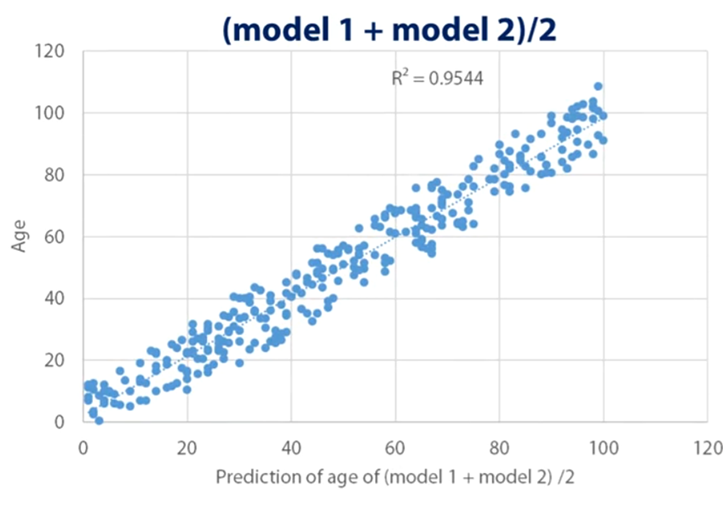
\includegraphics[width=0.7\linewidth]{./images/ensembling2.png} 
    \caption{Averaged Predictions: Better Correlation}
\end{figure}
\end{frame}

\begin{frame}{Ensembling}
\begin{itemize}
    \item Diverse models are key to effective ensembling. Here are two strategies:
    \begin{itemize}
        \item \textbf{Bagging (Bootstrap Aggregating):} Train multiple models on different subsets of data (e.g., Random Forest model).
    \end{itemize}
    \end{itemize}
    \begin{figure}
    \centering
    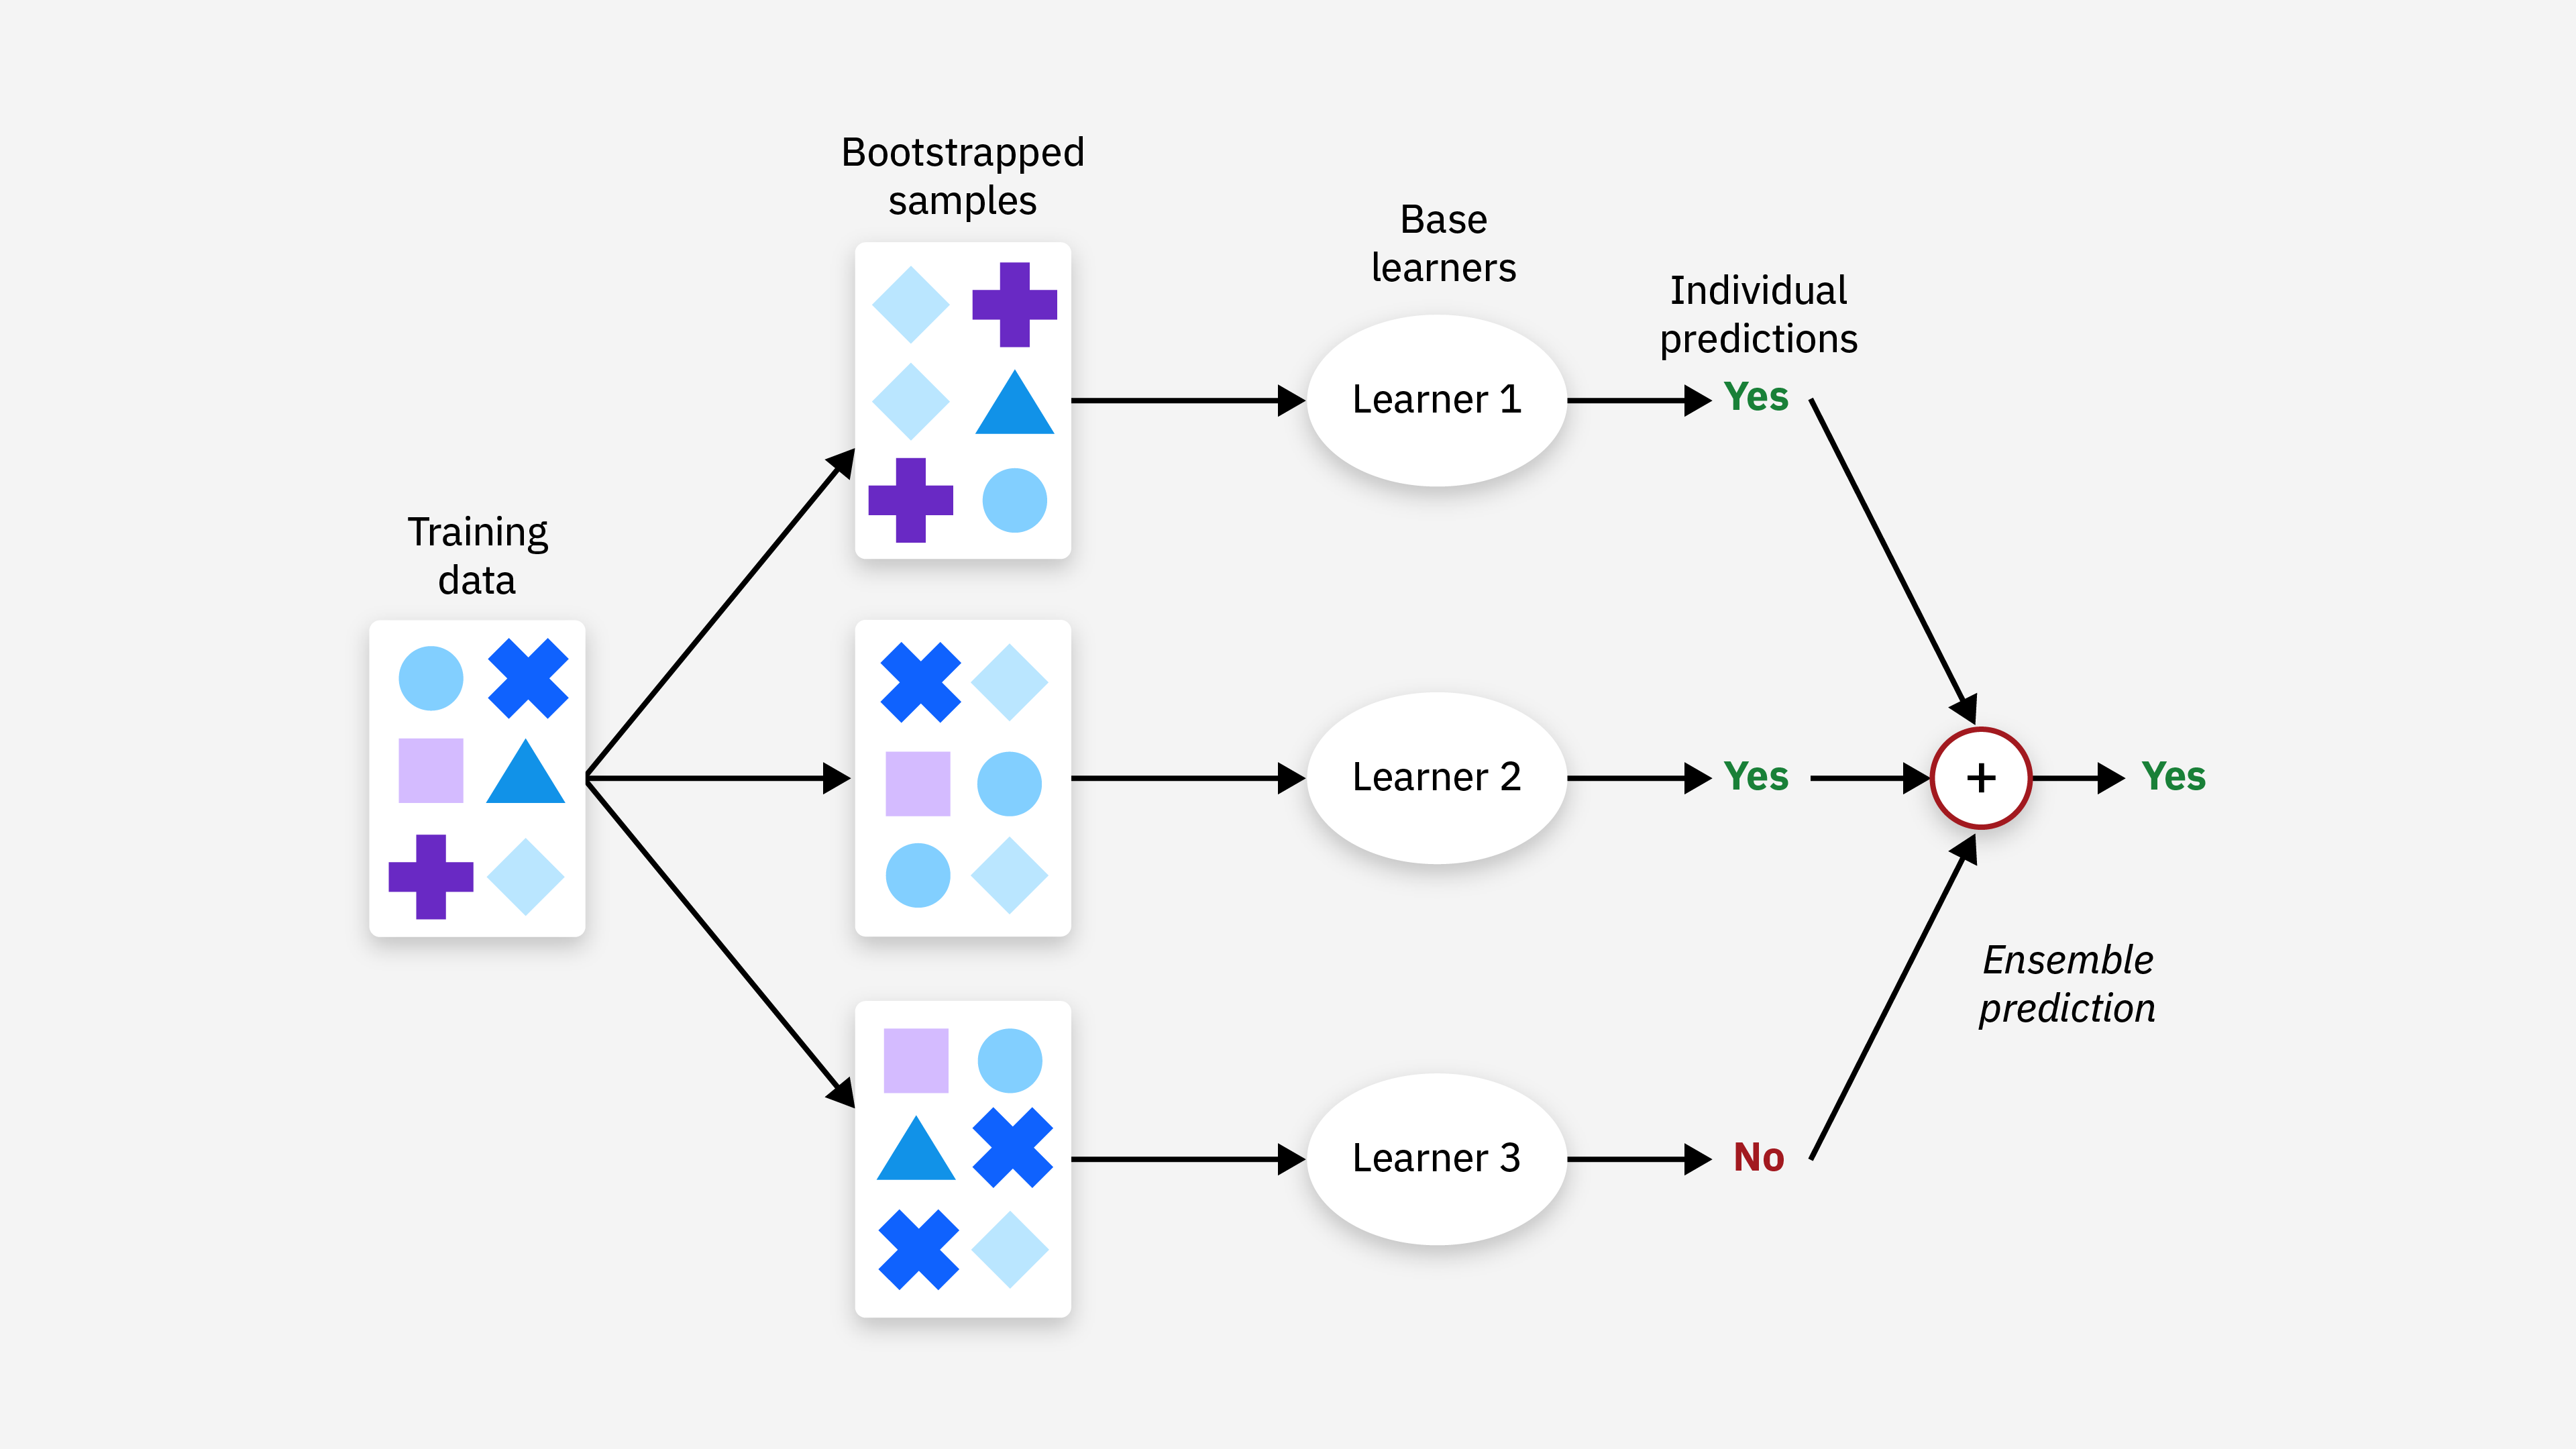
\includegraphics[width=0.8\textwidth,height=0.8\textheight,keepaspectratio]{./images/bagging.png}
    \caption{Bagging example}
\end{figure}
\end{frame}

\begin{frame}{Ensembling}
\begin{itemize}
    \begin{itemize}
        \item \textbf{Boosting:} Train models sequentially, where each model focuses on the errors of the previous one (e.g., AdaBoost, Gradient Boosting).
    \end{itemize}
    \end{itemize}
    \begin{figure}
    \centering
    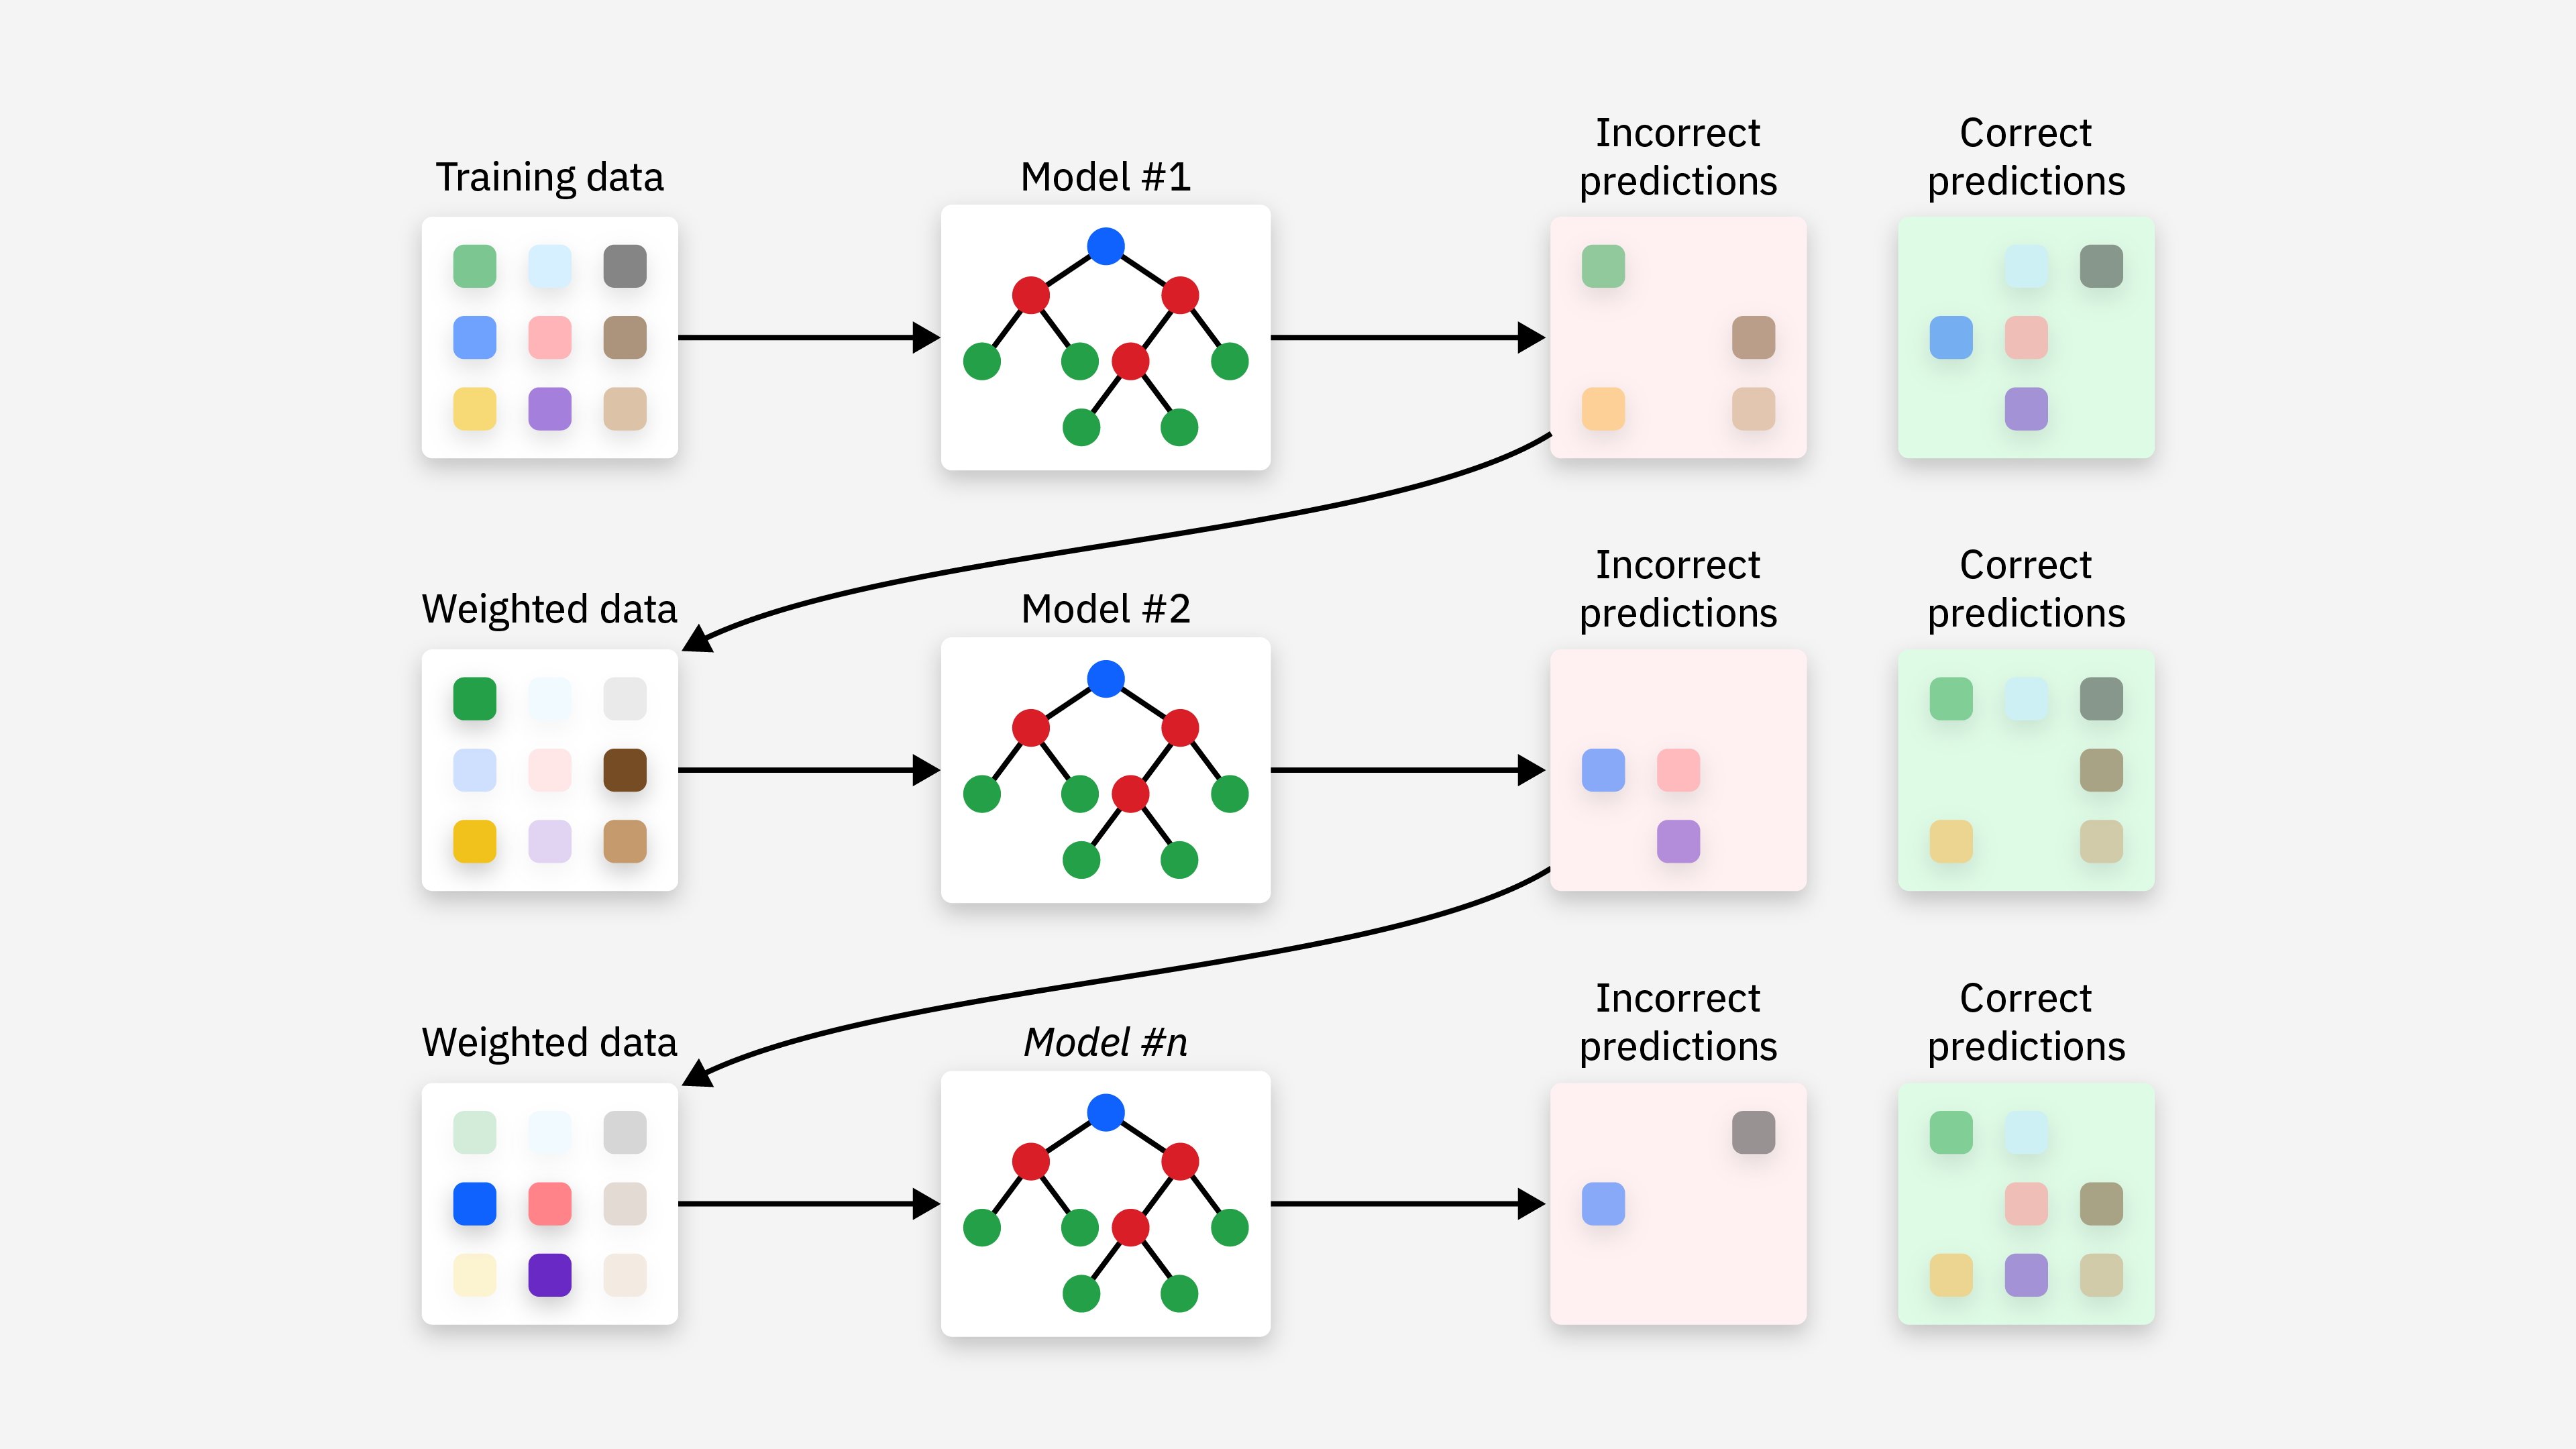
\includegraphics[width=0.8\textwidth,height=0.8\textheight,keepaspectratio]{./images/boosting.png}
    \caption{Boosting Example}
\end{figure}
\end{frame}

\begin{frame}{Ensembling}
\begin{itemize}
\item These stratigies introduce diversity in models, but how can we combine their predictions?
\end{itemize}
\end{frame}

\begin{frame}{Ensembling}
\begin{itemize}
\item We can combine classifiers predictions using two ways:
\begin{itemize}
    \item \textbf{Hard Voting:}
    \begin{itemize}
        \item Each model votes for a class.
        \item The class with the majority of votes is selected.
    \end{itemize}
    \item \textbf{Soft Voting:}
    \begin{itemize}
        \item Average the predicted probabilities from each model.
        \item The class with the highest average probability is selected.
    \end{itemize}
\end{itemize}
\end{itemize}
\begin{figure}
    \centering
    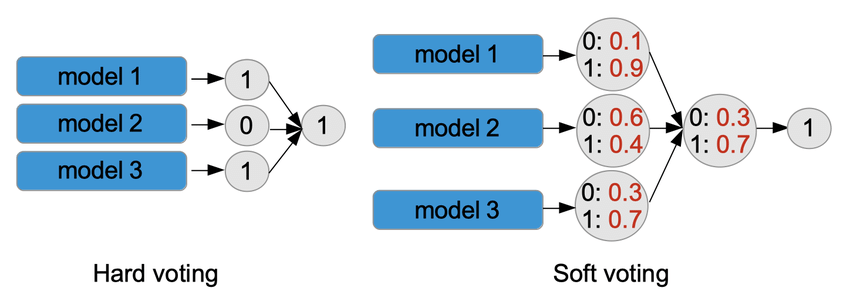
\includegraphics[width=0.8\linewidth]{./images/voting.png}
    \caption{Illustration of Hard and Soft Voting for Classifiers}
\end{figure}
\end{frame}



\begin{frame}{Ensembling}
\begin{itemize}
\item We can combine classifiers predictions using two ways:
\begin{itemize}
    \item \textbf{Hard Voting:}
    \begin{itemize}
        \item Each model votes for a class.
        \item The class with the majority of votes is selected.
    \end{itemize}
    \item \textbf{Soft Voting:}
    \begin{itemize}
        \item Average the predicted probabilities from each model.
        \item The class with the highest average probability is selected.
    \end{itemize}
\end{itemize}
\end{itemize}
\begin{itemize}
\item For regressors:
    \begin{itemize}
        \item Take the average of predictions from all models.
        \end{itemize}
\end{itemize}
\end{frame}


\begin{frame}{Ensembling}
    \begin{itemize}
        \item Team-work is the best policy.
        \item We can train multiple networks for the same task then ensemble to get better results.
    \end{itemize}

\end{frame}

% \begin{frame}{Bagging in Ensemble Learning}
% \begin{itemize}
%     \item \textbf{Bagging (Bootstrap Aggregating)} is a parallel ensemble learning method that improves model stability and accuracy by reducing variance.
%     \item It creates multiple training datasets by \textbf{bootstrap resampling}:
%     \begin{itemize}
%         \item Given a dataset with $n$ samples, multiple bootstrap samples of size $n$ are drawn with replacement.
%         \item Some instances appear multiple times, while others are omitted.
%     \end{itemize}
%     \item Each bootstrap sample is used to train an independent \textbf{base learner} (e.g., decision tree, neural network).
%     \item The final prediction is obtained through \textbf{majority voting} (classification) or \textbf{averaging} (regression).
% \end{itemize}

% \footnotetext{\href{https://www.ibm.com/think//ensemble-learning}{IBM: Ensemble Learning}}
% \end{frame}

% \begin{frame}{Bagging - Example: Random Forest}
% \begin{itemize}
%     \item \textbf{Random Forest} is a popular extension of bagging applied to decision trees.
%     \item Instead of considering all features at each split, \textbf{random subsets} of features are selected.
%     \item This introduces additional randomness, improving generalization and preventing overfitting.
%     \item Random forests outperform individual decision trees, especially on noisy datasets.
% \end{itemize}
% \footnotetext{\href{https://www.ibm.com/think/topics/ensemble-learning}{IBM: Ensemble Learning}}
% \end{frame}


% \begin{frame}{Bagging}
% \begin{figure}
%     \centering
%     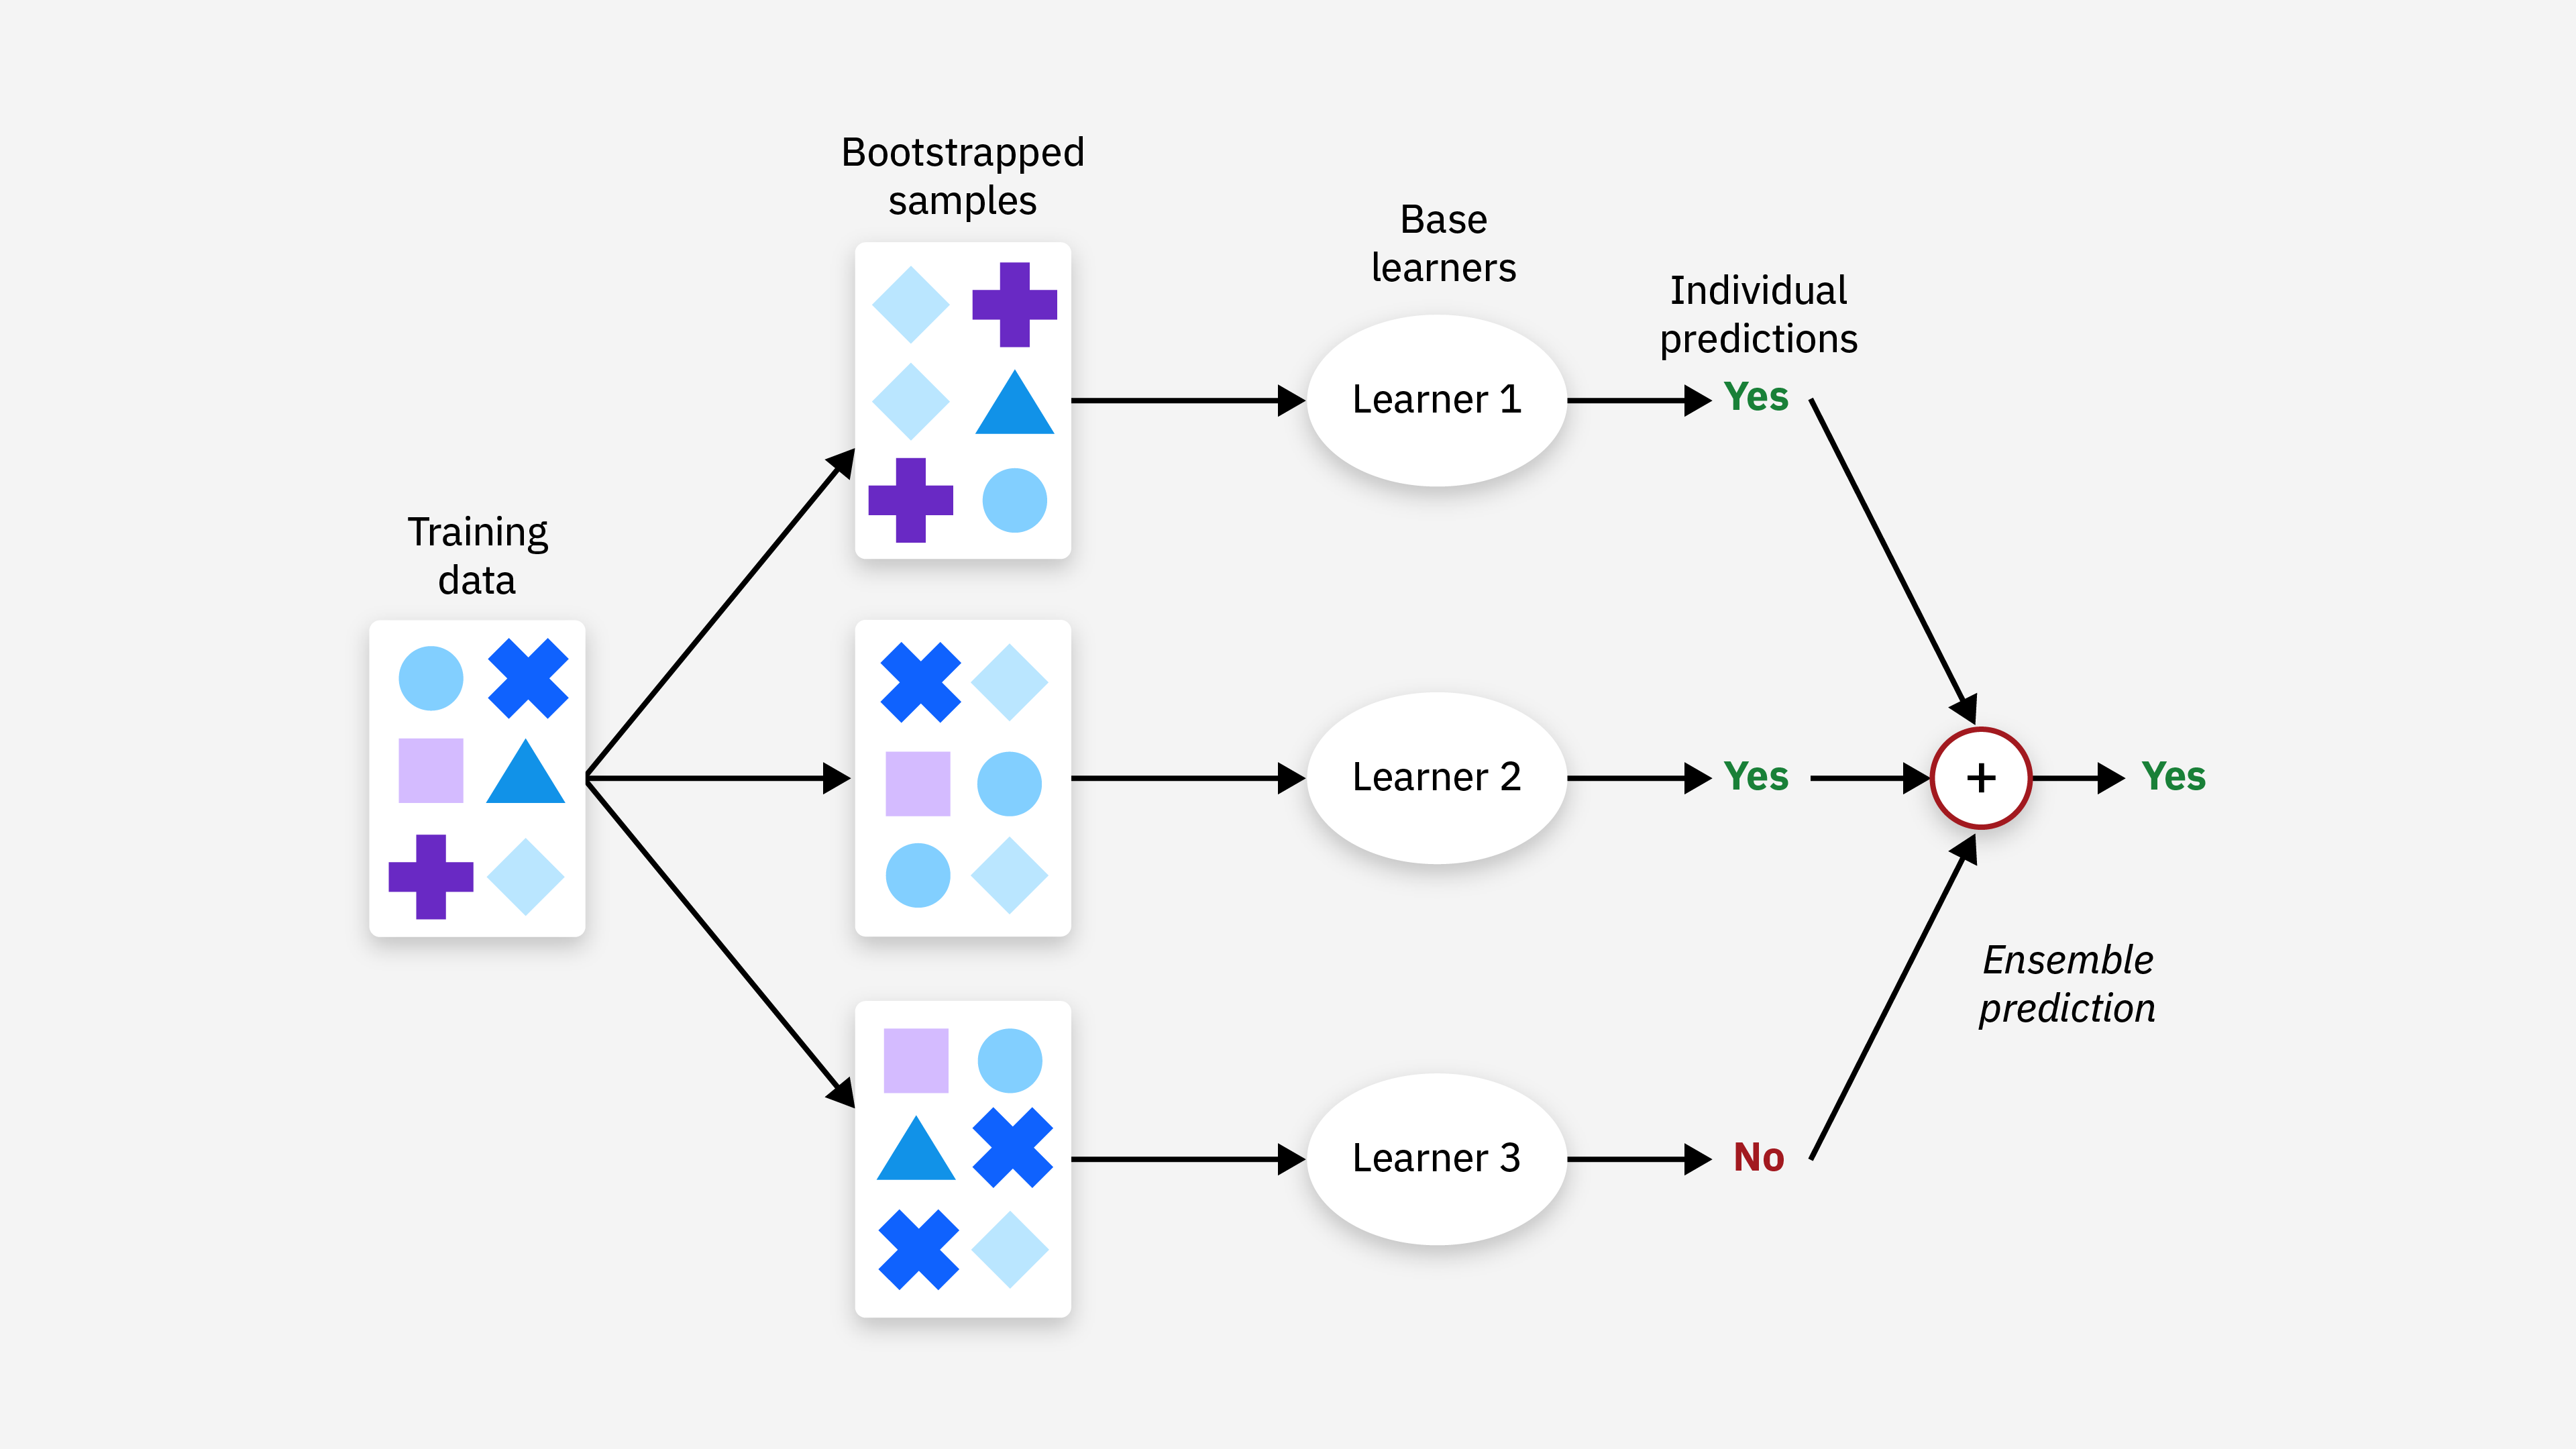
\includegraphics[width=1.0\textwidth,height=0.8\textheight,keepaspectratio]{./images/bagging.png}
%     \caption{Bagging example}
% \end{figure}
    
% \end{frame}


% \begin{frame}{Boosting in Ensemble Learning}
% \begin{itemize}
%     \item \textbf{Boosting} is a sequential ensemble learning method that builds strong models by correcting the mistakes of weaker ones.
%     \item Unlike bagging, where models are trained independently, boosting \textbf{trains learners sequentially}, prioritizing misclassified samples.
%     \item General process:
%     \begin{enumerate}
%         \item Train a weak model on the dataset $D_1$.
%         \item Identify misclassified instances and assign them higher weights.
%         \item Train a second model on a new dataset $D_2$, emphasizing difficult cases.
%         \item Repeat the process for $n$ iterations, gradually improving predictions.
%         \item Combine all models using weighted averaging or boosting-specific techniques.
%     \end{enumerate}
% \end{itemize}

% \footnotetext{\href{https://www.ibm.com/think/topics/ensemble-learning}{IBM: Ensemble Learning}}
% \end{frame}

% \begin{frame}{Types of Boosting Algorithms}
% \begin{itemize}
%     \item \textbf{Adaptive Boosting (AdaBoost)}:
%     \begin{itemize}
%         \item Assigns weights to misclassified samples to prioritize them in the next iteration.
%         \item Models are combined based on weighted majority voting.
%     \end{itemize}

%     \item \textbf{Gradient Boosting}:
%     \begin{itemize}
%         \item Instead of weighting misclassified samples, it minimizes residual errors by training new models to predict the previous model’s errors.
%         \item Used in advanced implementations like \textbf{XGBoost}, \textbf{LightGBM}, and \textbf{CatBoost}.
%     \end{itemize}
    
%     \item \textbf{Extreme Gradient Boosting (XGBoost)}:
%     \begin{itemize}
%         \item Optimized version of gradient boosting with parallel processing, tree pruning, and regularization.
%         \item One of the most widely used ML techniques in Kaggle competitions.
%     \end{itemize}
% \end{itemize}

% \footnotetext{\href{https://www.ibm.com/think/topics/ensemble-learning}{IBM: Ensemble Learning}}
% \end{frame}
% \begin{frame}{Boosting Example}
%     \begin{figure}
%     \centering
%     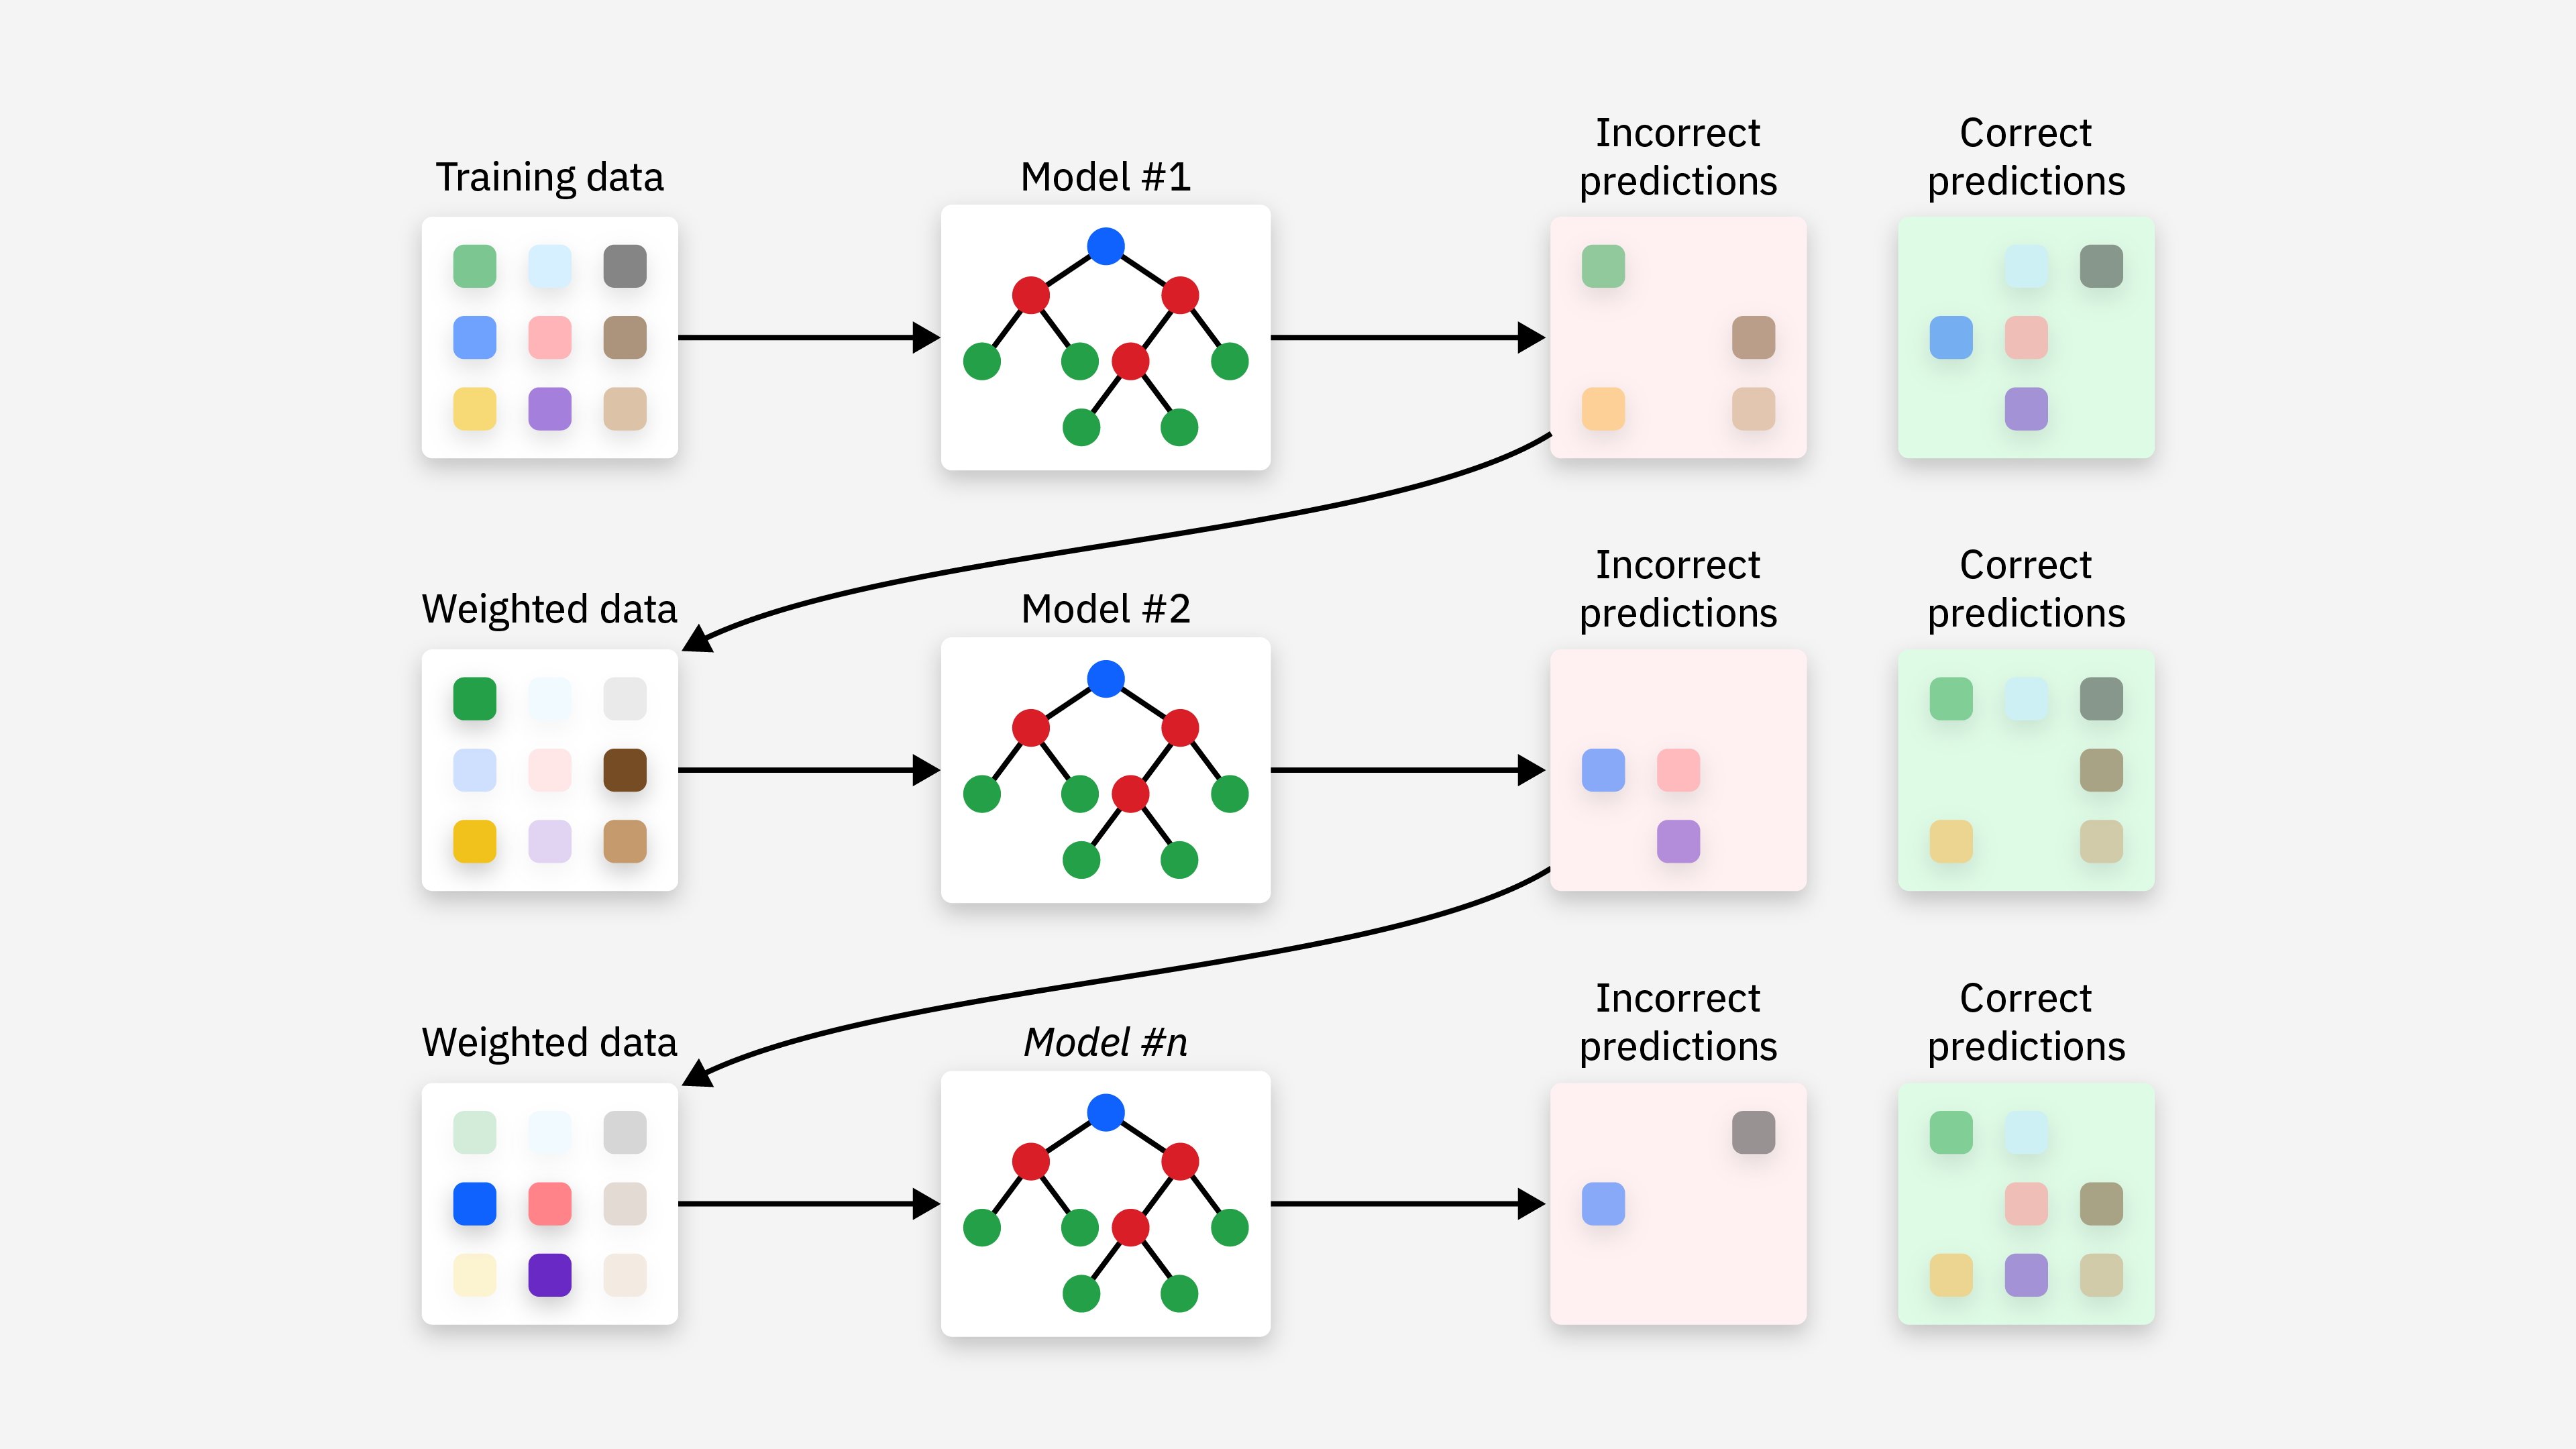
\includegraphics[width=1.0\textwidth,height=0.8\textheight,keepaspectratio]{./images/boosting.png}
%     \caption{Boosting Example}
% \end{figure}
% \end{frame}


% \begin{frame}{Boosting vs Bagging}
% \begin{itemize}
%     \item \textbf{Bagging} reduces variance by training multiple models independently on different bootstrapped datasets.
%     \item \textbf{Boosting} reduces bias by training models sequentially and focusing on misclassified instances.
%     \item Bagging (e.g., \textbf{Random Forest}) is effective for reducing overfitting.
%     \item Boosting (e.g., \textbf{XGBoost}, \textbf{AdaBoost}) works well for improving weak learners and tackling complex problems.
% \end{itemize}


% \footnotetext{\href{https://www.ibm.com/think/topics/ensemble-learning}{IBM: Ensemble Learning}}
% \end{frame}

\begin{frame}{Ensembling - A simple Analysis}
    
\begin{itemize}
    \item Let’s assume that we have a test dataset with $N$ elements and an ensemble of $M$ models.
    \item Also assume that the probability of error of the label for an image on a model in the ensemble is denoted by $p(e)$ and is Independent and Identically Distributed (i.i.d)
    \item For an example assume $M=3$ and $e =0.01$
    \item Then probability of error of label for the max voting ensemble will be
    $$p(e) = 1 - (1-e)^3 - \binom 32 (1-e)^2 e$$
    \item For the above example $p(e)=0.0003$, which is significantly lower than a single model
\end{itemize}
\end{frame}

\begin{frame}{Dropout}
    \begin{itemize}
    \item \textbf{Dropout} is a regularization technique used to prevent overfitting in neural networks.
    \item During training, it randomly drops (set to 0) a fraction of neurons in each layer based on a specified probability for every forward pass.
\end{itemize}
    \begin{figure}
    \centering
    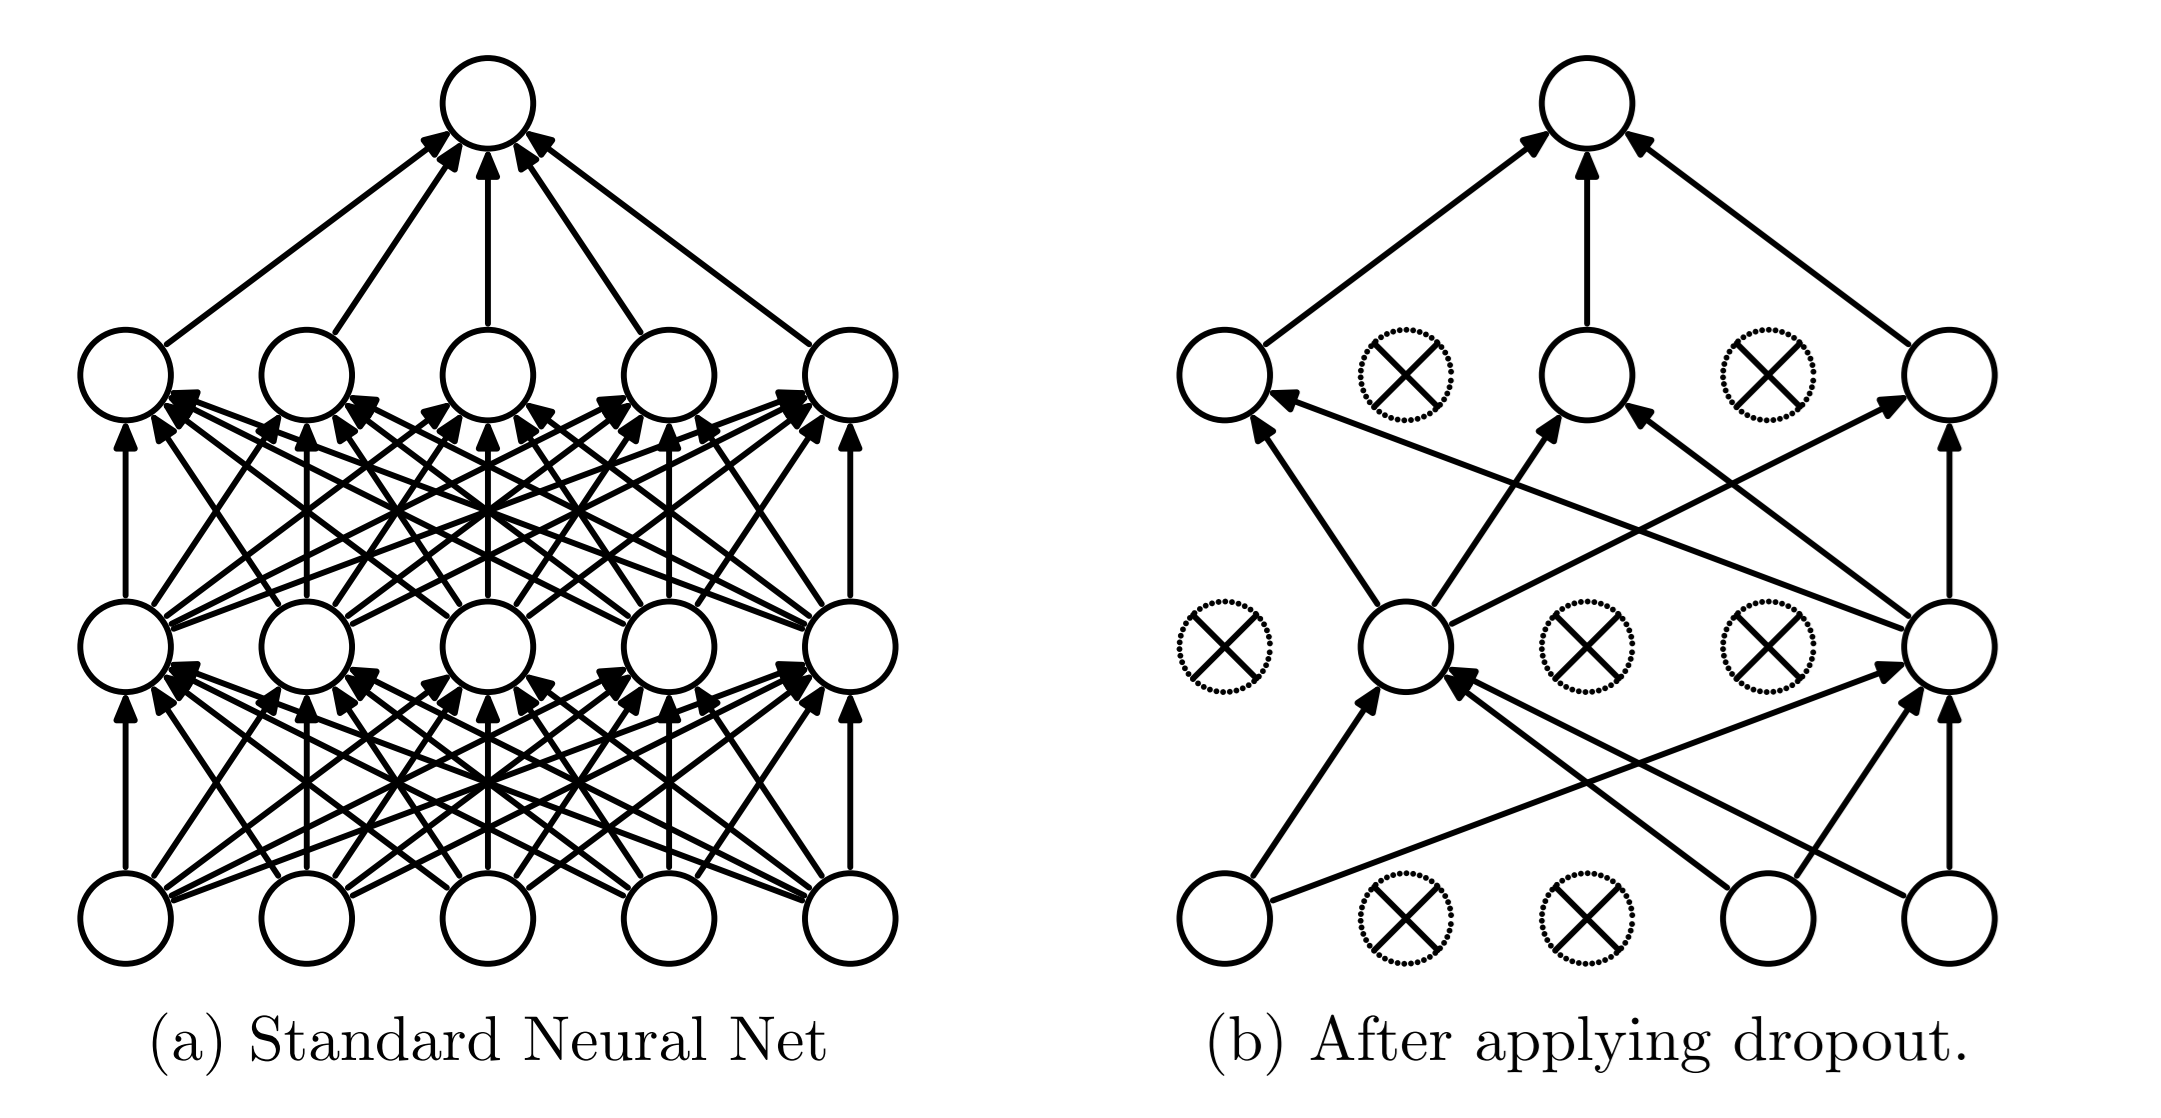
\includegraphics[width=0.8\textwidth,height=0.8\textheight,keepaspectratio]{./images/dropout_1.png}
    \end{figure}
\footnotetext{\href{https://jmlr.org/papers/volume15/srivastava14a/srivastava14a.pdf}{Srivastava JMLR 2014}}
\end{frame}

\begin{frame}{Dropout}
\begin{itemize}
    \item Why is dropping neurons randomly useful?
\begin{enumerate}
    \item By dropping a subset of neurons during each forward pass, the network learns \textbf{not to rely too heavily on specific connections}, encouraging the network to use more connections.
 
    \item Dropout acts as an \textbf{efficient ensemble} of multiple smaller networks, each trained on a random subset of neurons.
    \item More Connections + Diverse Ensemble = \textbf{less overfitting}.
\end{enumerate}
\end{itemize}
\end{frame}

\begin{frame}{Dropout}
    \begin{figure}
    \centering
    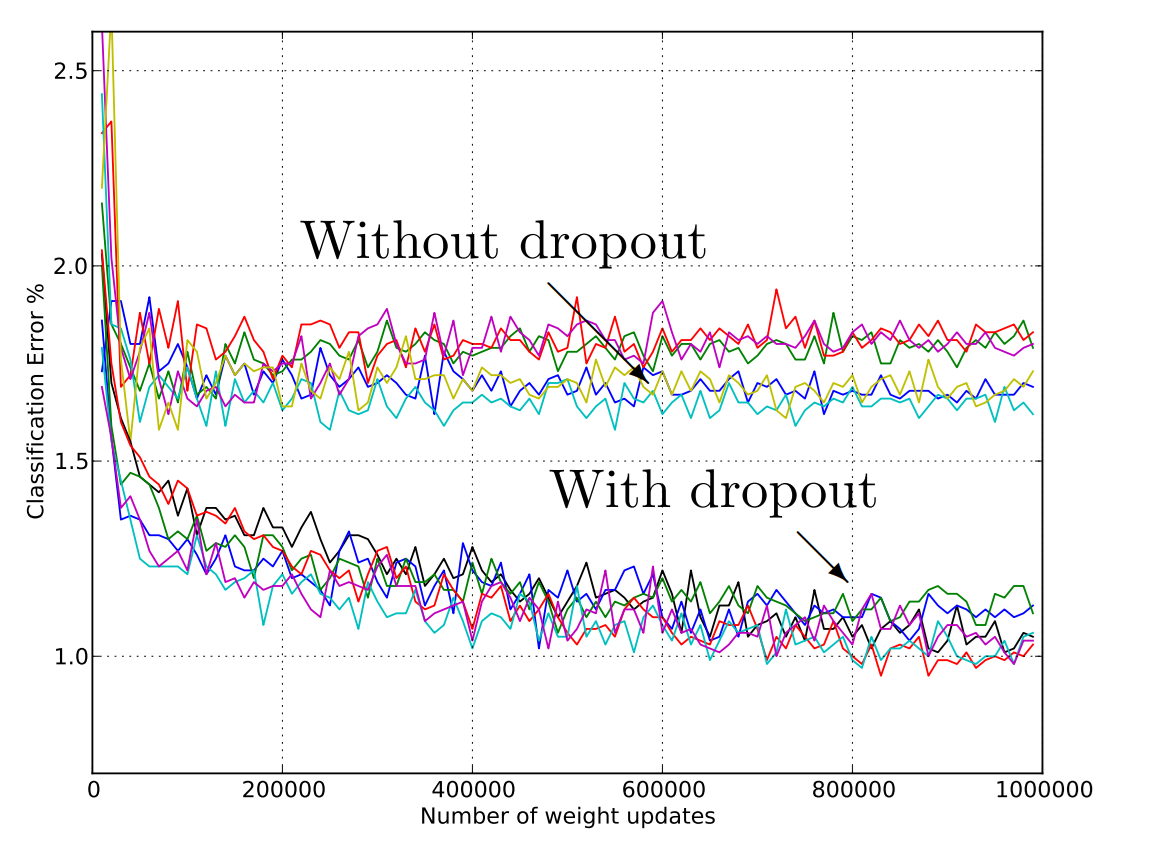
\includegraphics[width=1.0\textwidth,height=0.5\textheight,keepaspectratio]{./images/dropout_3.png}
    \end{figure}

    \begin{figure}
    \centering
    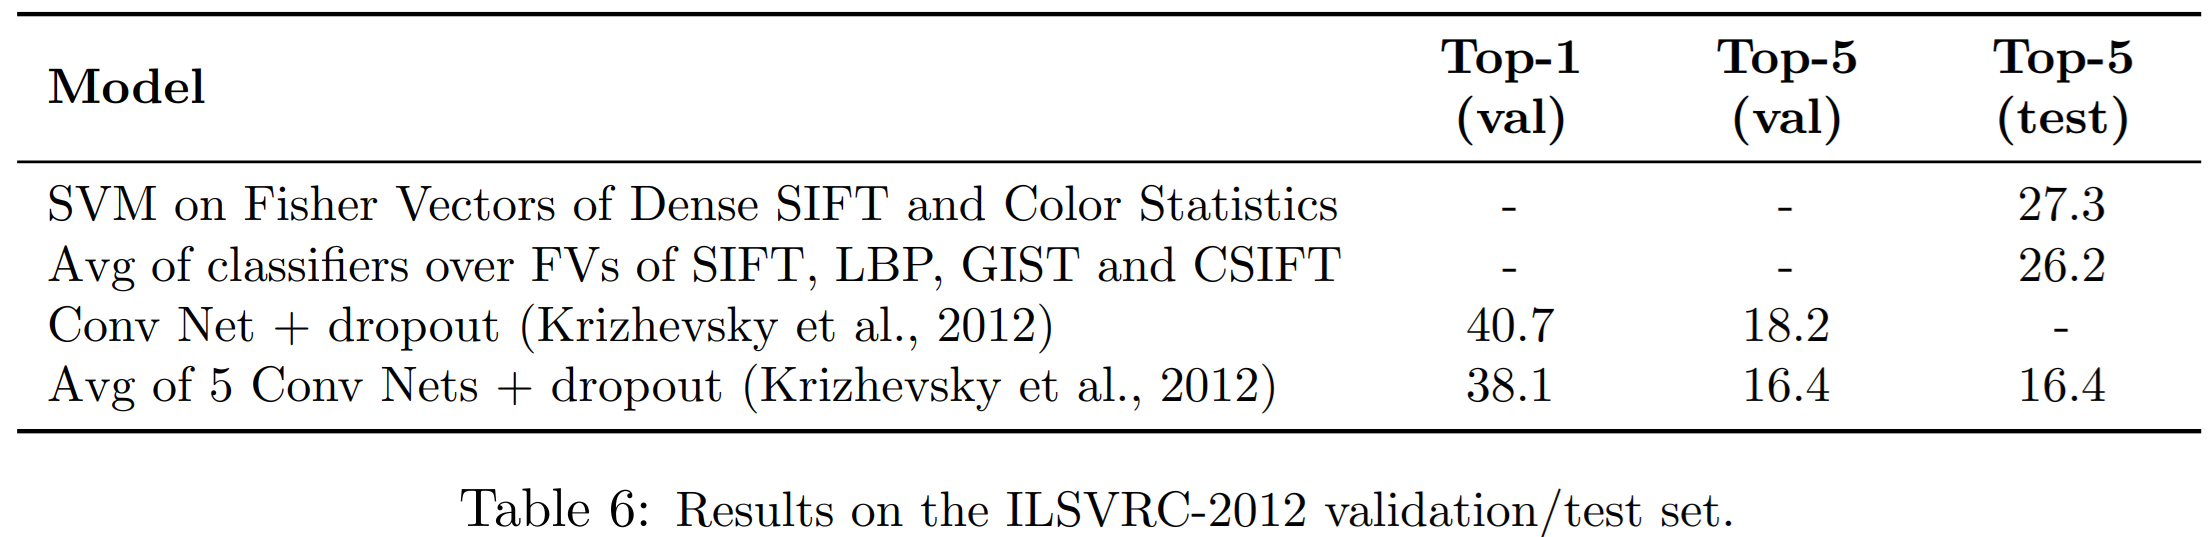
\includegraphics[width=1.0\textwidth,height=0.5\textheight,keepaspectratio]{./images/dropout_4.png}
    \end{figure}
\footnotetext{\href{https://jmlr.org/papers/volume15/srivastava14a/srivastava14a.pdf}{Srivastava JMLR 2014}}

\end{frame}

\begin{frame}{Dropout}
\begin{itemize}
    \item We drop neurons during training, but what should we do during inference?
    \item \textbf{During inference:} We use all neurons. 

    \begin{figure}
    \centering
    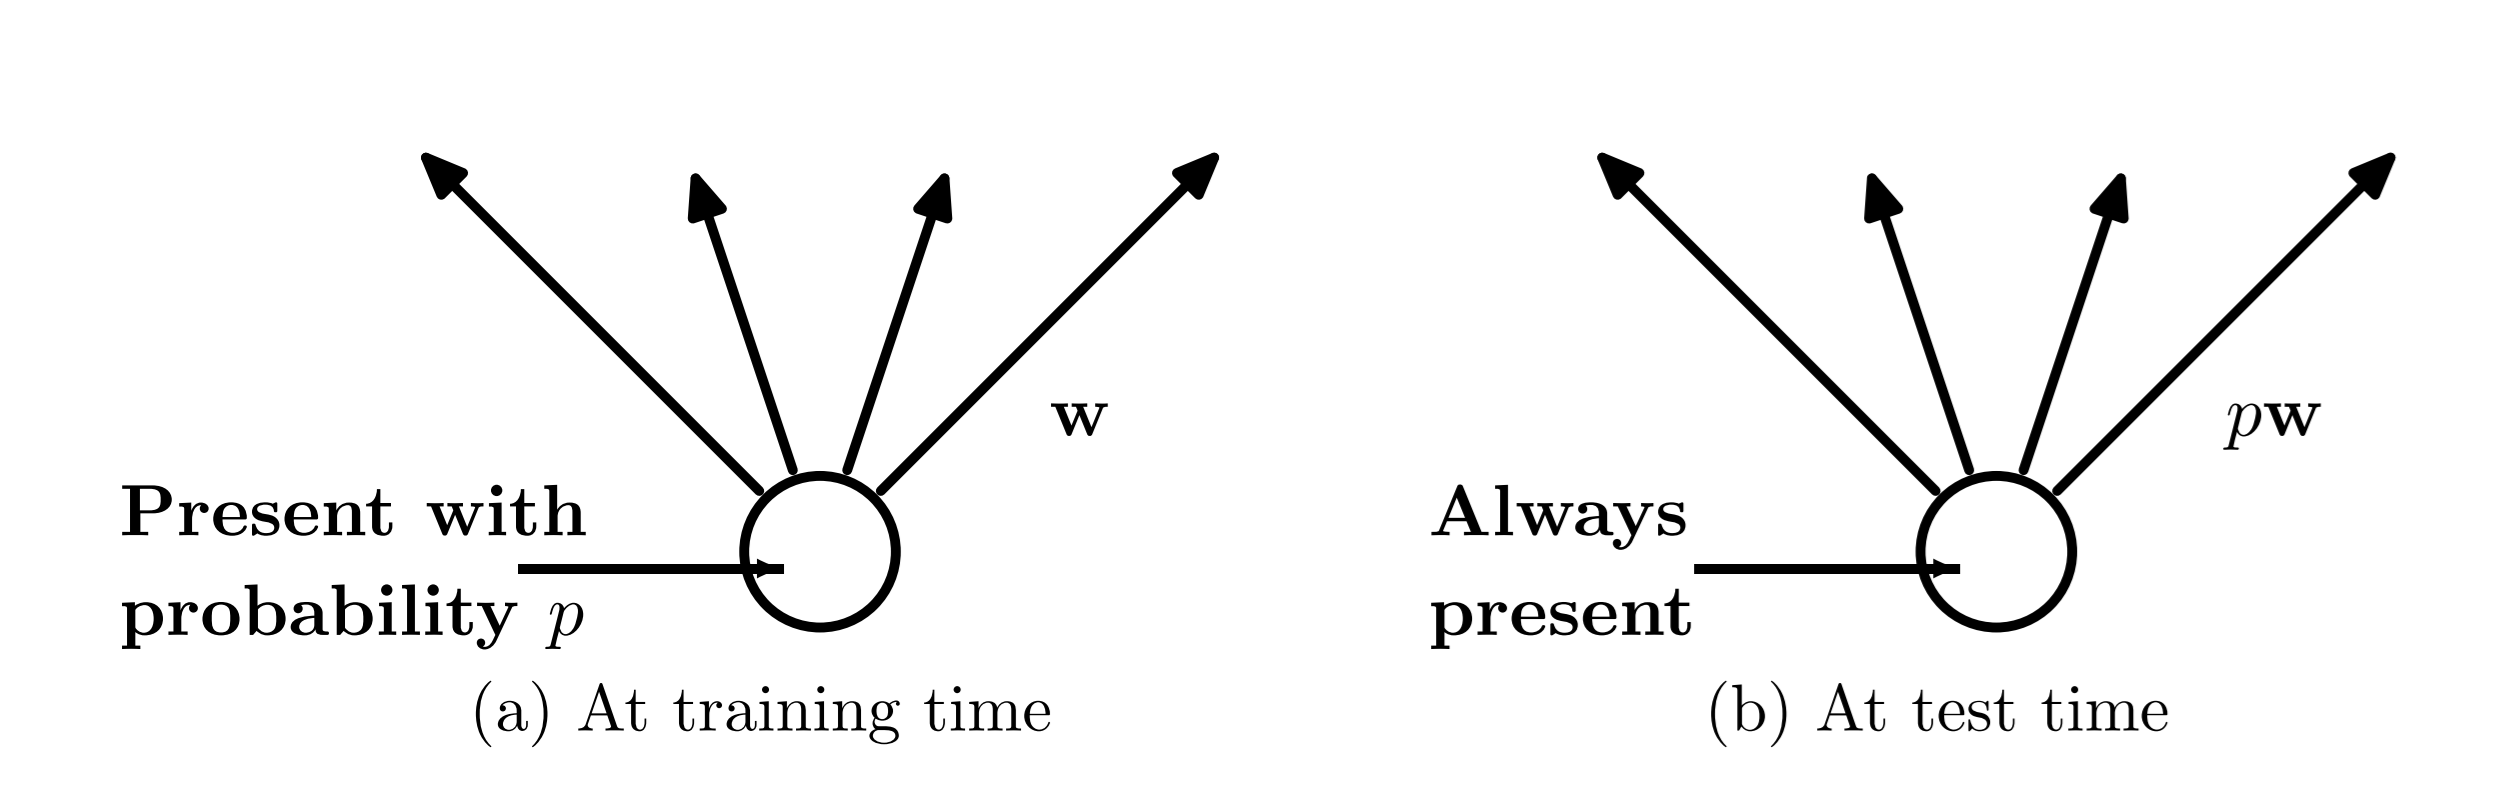
\includegraphics[width=1.0\textwidth,height=0.8\textheight,keepaspectratio]{./images/dropout_2.png}
    \end{figure}
\footnotetext{\href{https://jmlr.org/papers/volume15/srivastava14a/srivastava14a.pdf}{Srivastava JMLR 2014}}

\item but... 

    
\end{itemize}
\end{frame}

\begin{frame}{Dropout}
\begin{figure}
    \centering
    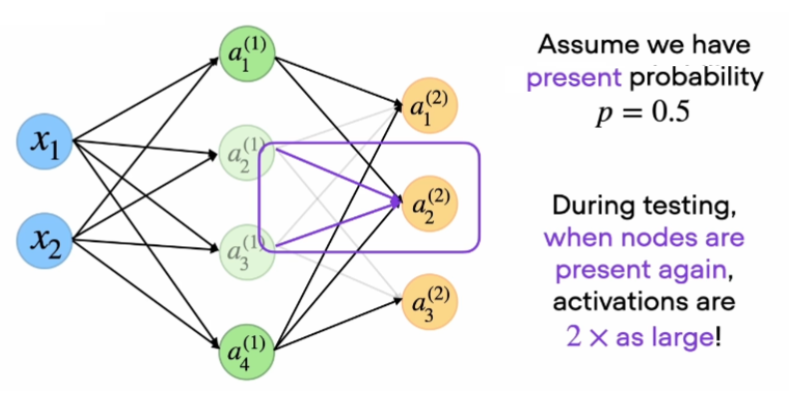
\includegraphics[width=1.0\textwidth,height=1.0\textheight,keepaspectratio]{./images/dropout_light.png}
    \end{figure}
    \footnotetext{\href{https://lightning.ai/courses/deep-learning-fundamentals}{Deep Learning Fundamentals - Lightning AI}}
\end{frame}

\begin{frame}{Dropout}
\begin{itemize}
    \item \textbf{Problem:} Having inconsistent values during inference compared to training can cause the network to produce worse results.
    \item \textbf{Solution:} Scale the output during inference by \(p\) to keep the same expected activation as in training.
    \item \textbf{Example:}
    \begin{itemize}
  \item \textbf{During training (p=0.1)}: 
    \begin{itemize}
      \item Activation value = 2
      \item Active only 10\% of the time 
      \item \(\Rightarrow\) Effective contribution = \(2 \times 0.1 = 0.2\)
    \end{itemize}
  \item \textbf{During inference}: 
    \begin{itemize}
      \item Always active (\(\Rightarrow\) Activation value = 2)
      \item Scale by \((p) = 0.1\)
      \[
        2 \times 0.1 = 0.2
      \]
    \end{itemize}
  \item Result: Consistent activation scale between training and inference.
\end{itemize}

\end{itemize}
\end{frame}


\begin{frame}{Dropout}
    \begin{itemize}
        \item In PyTorch, dropout behavior is controlled by the model's mode:
            \begin{block}{}
        \texttt{\small
        \# Training Mode: Enables dropout\\
        model.train() \\
        output = model(input) \\
        \\
        \# Evaluation Mode: Disables dropout, scales activations\\
        model.eval() \\
        output = model(input)
        }
    \end{block}

    \end{itemize}


\end{frame}


% \begin{frame}{Dropout}
%     \begin{figure}
%     \centering
%     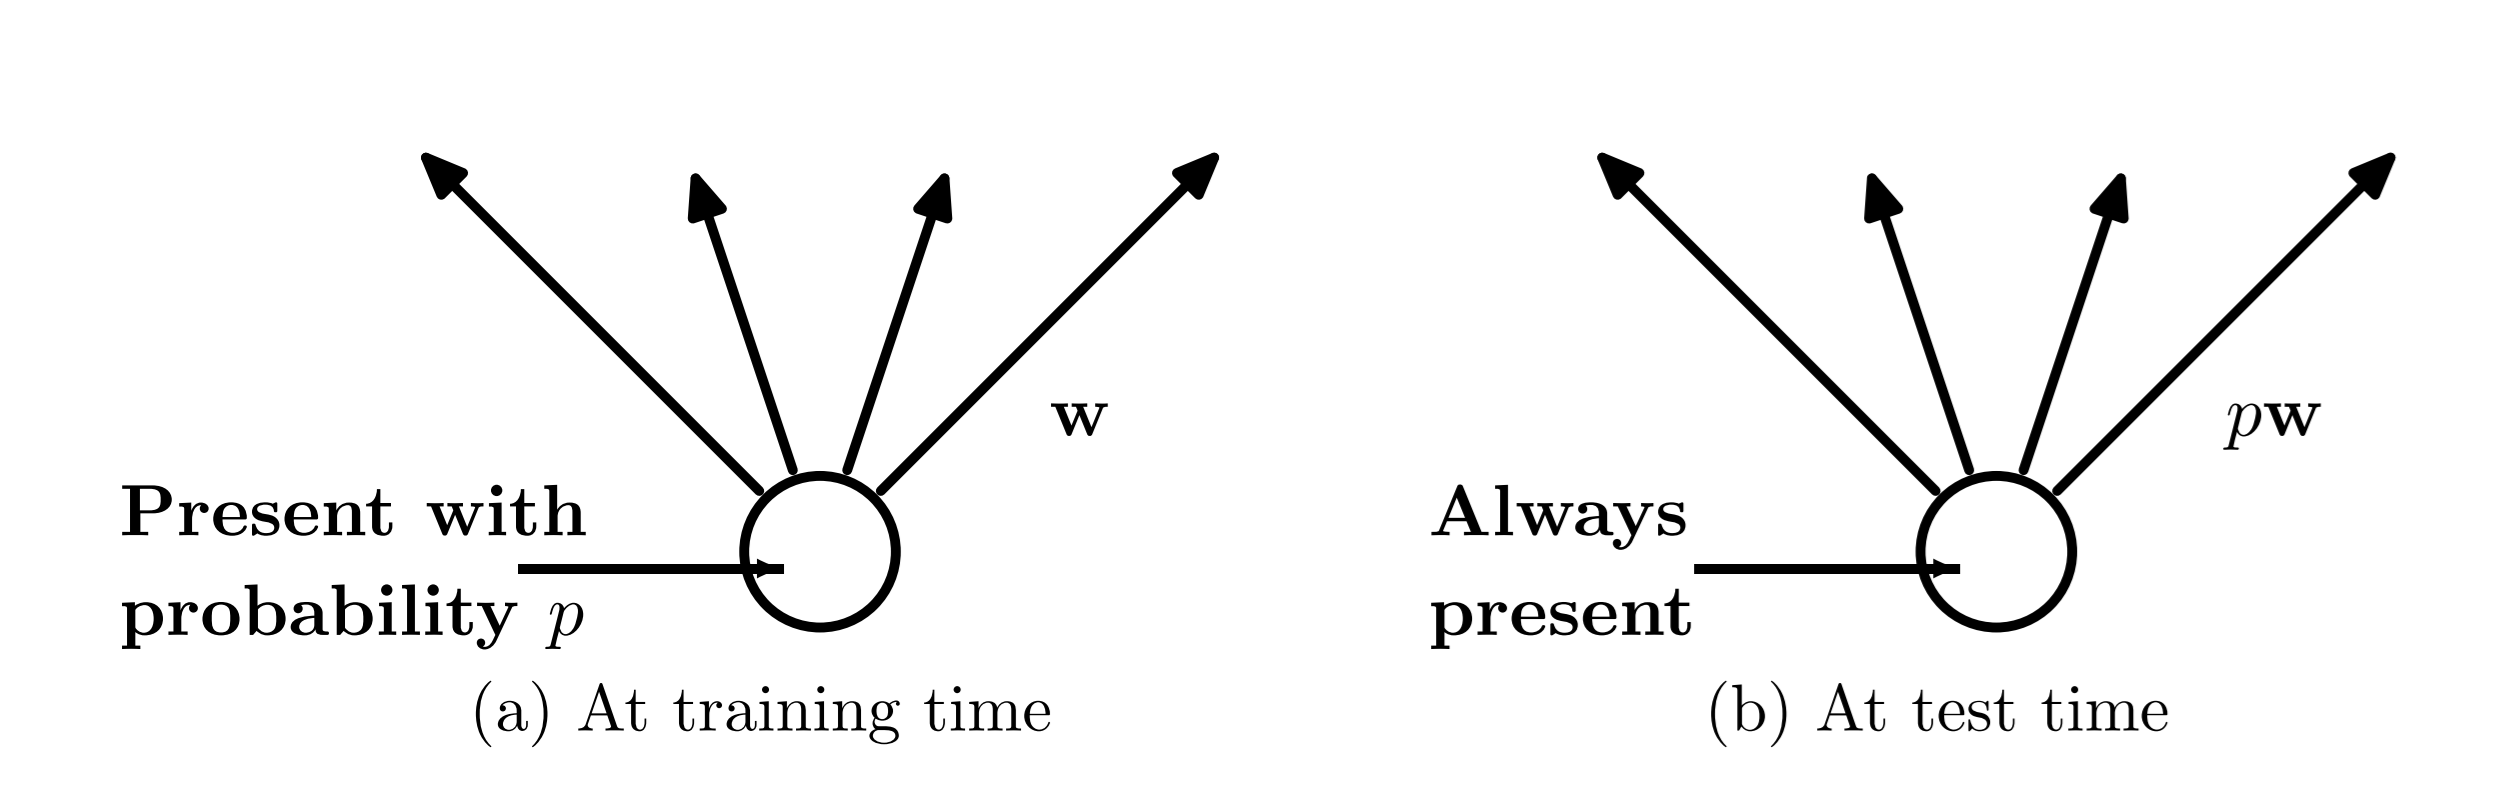
\includegraphics[width=1.0\textwidth,height=0.25\textheight,keepaspectratio]{./images/dropout_2.png}
%     \end{figure}
% \footnotetext{\href{https://jmlr.org/papers/volume15/srivastava14a/srivastava14a.pdf}{Srivastava JMLR 2014}}

% \textbf{Intuition:} successful conspiracies
% \begin{itemize}
%     \item 50 people planning a conspiracy
%     \item Strategy A: plan a big conspiracy involving 50 people
%     \begin{itemize}
%         \item Likely to fail. 50 people need to play their parts correctly.
%     \end{itemize}
%     \item Strategy B: plan 10 conspiracies each involving 5 people
%     \begin{itemize}
%         \item Likely to succeed!
%     \end{itemize}
% \end{itemize}
% \textbf{Main Idea:} approximately combining exponentially many different neural network architectures efficiently


% \end{frame}



\begin{frame}{Batch Normalization}
    \begin{itemize}
        \item \textbf{Key Insight}: Networks train better when inputs are normalized
        \item So why not normalize intermediate layers too?
        \item \textbf{Problem}: forcing every layer to output zero-mean, unit-variance values might be too restrictive (not always optimal).
        \item \textbf{Solution}: Let the network learn if it wants normalization!
    \end{itemize}
\end{frame}

\begin{frame}{Batch Normalization}
    For each feature in a layer:
    \begin{enumerate}
        \item First normalize: $\hat{x} = \frac{x - \mu}{\sqrt{\sigma^2 + \epsilon}}$
        \begin{itemize}
            \item $\mu$: mean across batch dimension
            \item $\sigma^2$: variance across batch dimension
            \item Computed separately for each feature/channel
        \end{itemize}
        \vspace{0.5em}
        \item Then give the network control:
        $y = \gamma\hat{x} + \beta$
        \begin{itemize}
            \item $\gamma$ (scale): Can amplify or reduce the normalized values
            \item $\beta$ (shift): Can move the values away from zero
            \item These are learned during training like normal weights!
        \end{itemize}
        
    \end{enumerate}
\end{frame}

\begin{frame}{Why $\gamma$ and $\beta$ Matter}
    \begin{itemize}
        \item After normalization, outputs are always zero-mean, unit-variance
        \item But this might not be optimal for every layer!
        \item $\gamma$ and $\beta$ let each layer learn:
        \begin{itemize}
            \item $\gamma$: "How much variance do I want?"
            \item $\beta$: "What should my mean activation be?"
        \end{itemize}
        \item Two extremes the network can learn:
        \begin{itemize}
            \item "Keep normalization": $\gamma \approx 1$, $\beta \approx 0$
            \item "Undo normalization": $\gamma$ and $\beta$ restore original scale and shift
        \end{itemize}
        \item Network learns what's best for each layer!
    \end{itemize}
\end{frame}

\begin{frame}{Batch Normalization}
    Mathematically, for batch size $N$, at each feature/channel $j$:
    \[
    \begin{aligned}
    \mu_j &= \frac{1}{N}\sum_{i=1}^N x_{i,j} \quad \text{(batch mean)} \\
    \sigma^2_j &= \frac{1}{N}\sum_{i=1}^N (x_{i,j} - \mu_j)^2 \quad \text{(batch variance)} \\
    \hat{x}_{i,j} &= \frac{x_{i,j} - \mu_j}{\sqrt{\sigma^2_j + \epsilon}} \quad \text{(normalize)} \\
    y_{i,j} &= \gamma_j\hat{x}_{i,j} + \beta_j \quad \text{(learnable transform)}
    \end{aligned}
    \]
\end{frame}

\begin{frame}{Batch Normalization}
    \begin{itemize}
        \item During Training:
        \begin{itemize}
            \item Use statistics from current batch
            \item Keep running average of mean and variance (to use later in inference): \\
            $\mu_{running} = 0.9 \times \mu_{running} + 0.1 \times \mu_{batch}$
        \end{itemize}
        \vspace{0.5em}
        \item During Inference (We can't depend on mini-batches):
        \begin{itemize}
            \item Use stored running averages ($\mu_{running}$, $\sigma^2_{running}$)
            \item These are fixed values from training
            \item No batch statistics needed!
        \end{itemize}
    \end{itemize}
\end{frame}

\begin{frame}{Batch Normalization}
    \begin{figure}
    \centering
    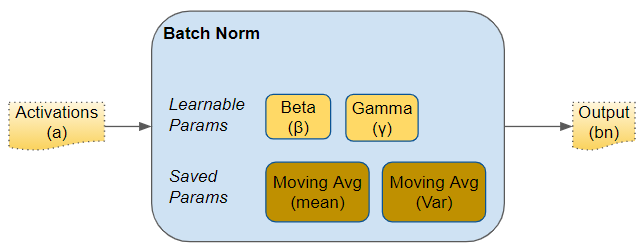
\includegraphics[width=1.0\textwidth,height=1.0\textheight,keepaspectratio]{./images/BatchNorm1.png}
    \end{figure}
    \footnotetext{\href{https://towardsdatascience.com/batch-norm-explained-visually-how-it-works-and-why-neural-networks-need-it-b18919692739/}{Ketan Doshi}}
\end{frame}

% \begin{frame}{Batch Normalization}
%     \begin{figure}
%     \centering
%     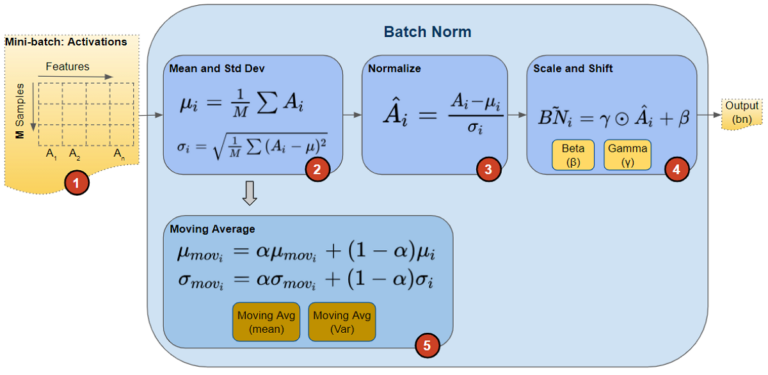
\includegraphics[width=1.0\textwidth,height=1.0\textheight,keepaspectratio]{./images/BatchNorm2.png}
%     \end{figure}
%     \footnotetext{\href{https://towardsdatascience.com/batch-norm-explained-visually-how-it-works-and-why-neural-networks-need-it-b18919692739/}{Ketan Doshi}}

% \end{frame}


% \begin{frame}{Batch Normalization}
%     \begin{figure}
%     \centering
%     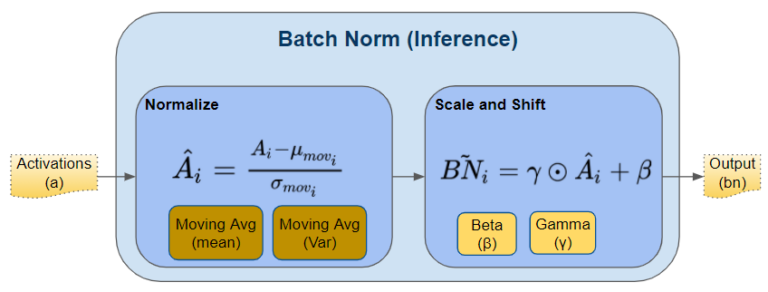
\includegraphics[width=1.0\textwidth,height=1.0\textheight,keepaspectratio]{./images/BatchNorm3.png}
%     \end{figure}
%     \footnotetext{\href{https://towardsdatascience.com/batch-norm-explained-visually-how-it-works-and-why-neural-networks-need-it-b18919692739/}{Ketan Doshi}}

% \end{frame}


\begin{frame}{Batch Normalization}
\begin{figure}
\centering
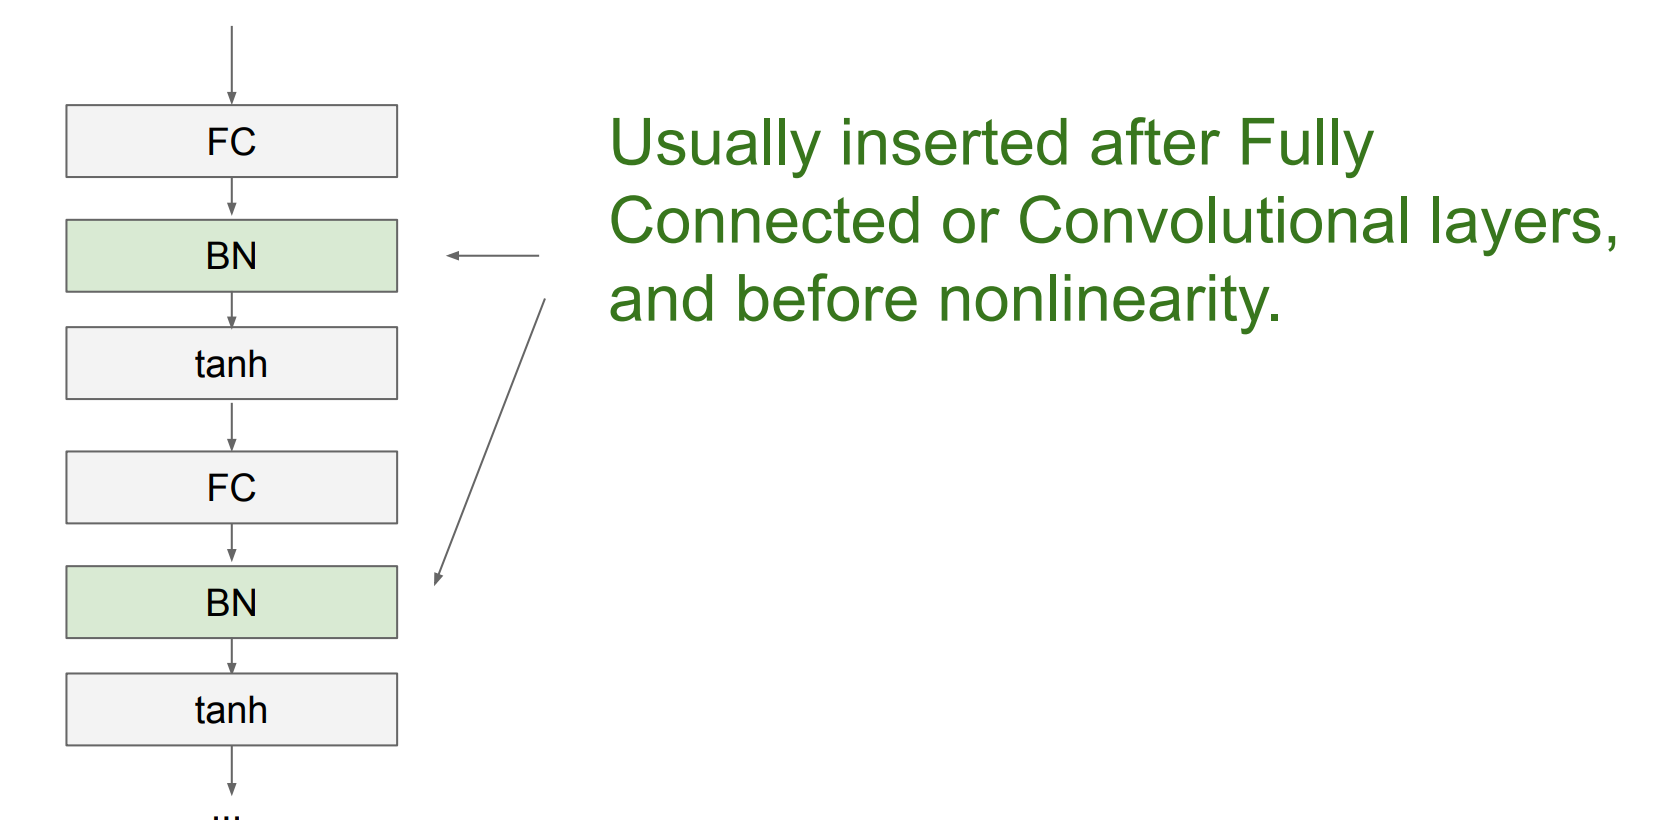
\includegraphics[width=1.0\textwidth,height=0.9\textheight,keepaspectratio]{./images/bn4.png}
\end{figure}
\footnotetext{\href{https://towardsdatascience.com/batch-norm-explained-visually-how-it-works-and-why-neural-networks-need-it-b18919692739/}{Ioffe and Szegedy 2015}}

\end{frame}


\begin{frame}{Batch Normalization}
    \begin{itemize}
        \item In Pytorch, batch normalization behavior is controlled by model's mode:
            \begin{block}{}
        \texttt{\small
        \# Training Mode: Use batch statistics\\
        model.train() \\
        output = model(input) \\
        \\
        \# Evaluation Mode: Use running statistics\\
        model.eval() \\
         output = model(input)
        }
    \end{block}
    \end{itemize}
\end{frame}



% \begin{frame}{Batch Normalization}
% \begin{itemize}
%     \item Consider a single layer $y=Wx$
%     \item The following could lead to tough optimazation
%     \begin{itemize}
%         \item Inputs $x$ are not centered around zero (need large bias)
%         \item Inputs $x$ have different scaling per element (entries in $W$ will need to vary a lot)
%     \end{itemize}
%     \pause
%     \item \textbf{Idea:} Force inputs to be "nicely scaled" at each layer!
% \end{itemize}
% \footnotetext{Slide based on CS231n by Fei-Fei Li, Yunzhu Li \& Ruohan Gao}
    
% \end{frame}

% \begin{frame}{Batch Normalization}
% \begin{itemize}
%     \item Consider a batch of activations at some layer. To make each dimension zero-mean unit-variance, apply:
%     $$\hat{x}^{(k)} = \frac{x^{(k)} - E[x^{(k)}]}{\sqrt{Var[x^{(k)}]}}$$
%     \pause
%     \item \textbf{Problem:} What if zero-mean, unit variance is too hard of a constraint?
% \end{itemize}
% \footnotetext{Slide based on CS231n by Fei-Fei Li, Yunzhu Li \& Ruohan Gao}
% \end{frame}

% \begin{frame}{Batch Normalization}
% \begin{figure}
% \centering
% 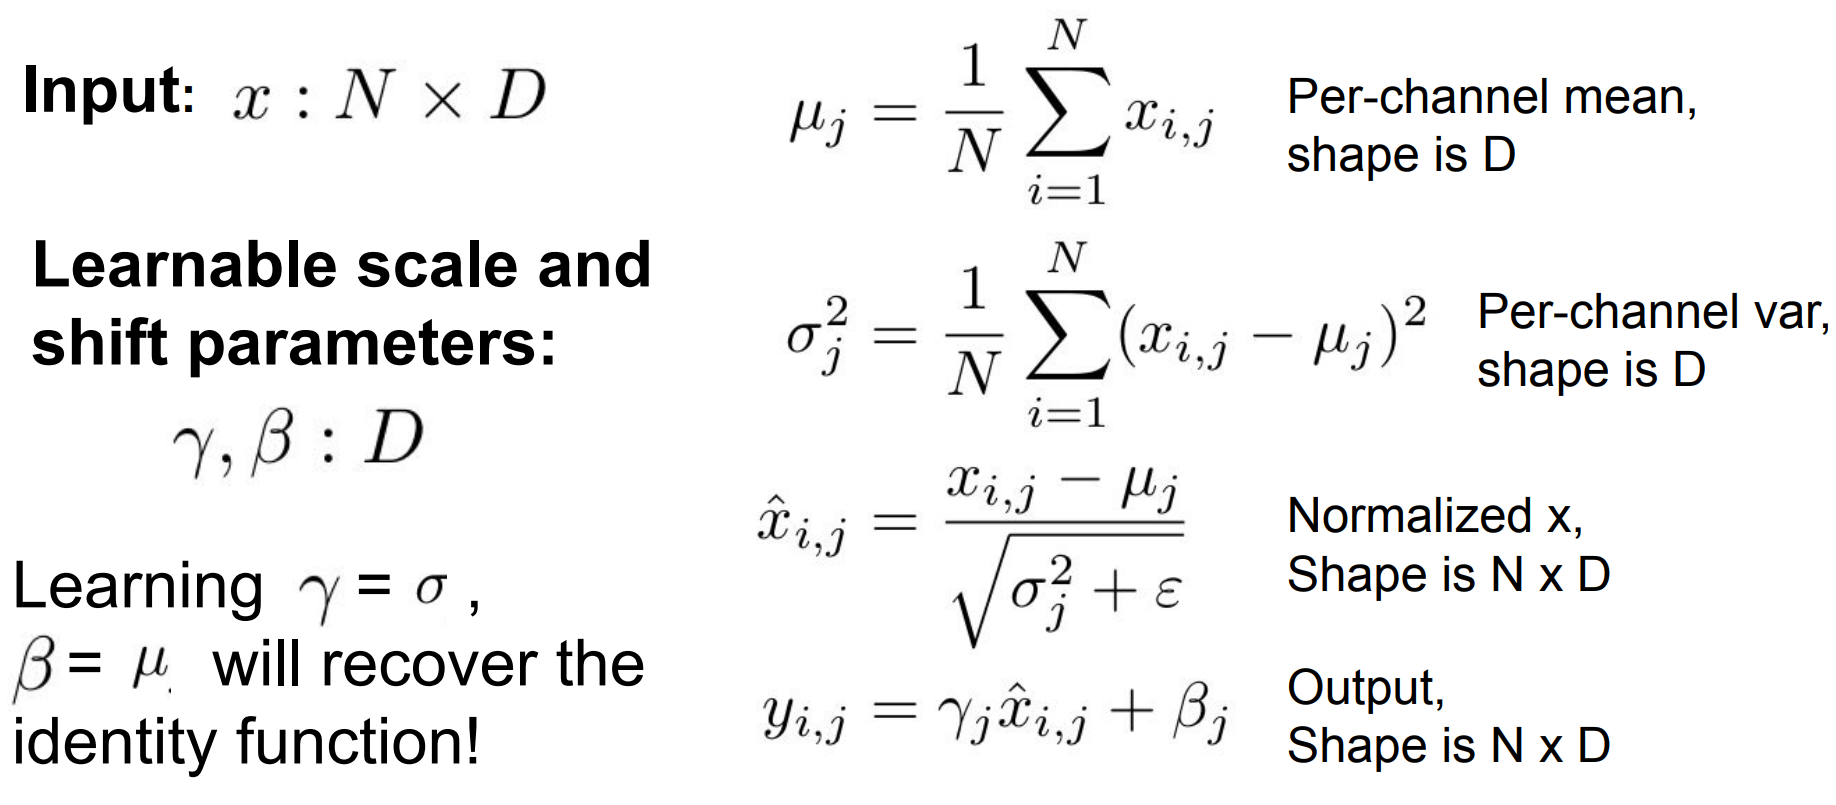
\includegraphics[width=1.0\textwidth,height=0.9\textheight,keepaspectratio]{./images/batch_norm_1.png}
% \end{figure}
% \footnotetext{Slide based on CS231n by Fei-Fei Li, Yunzhu Li \& Ruohan Gao}
% \end{frame}

% \begin{frame}{Batch Normalization}
% \begin{figure}
% \centering
% 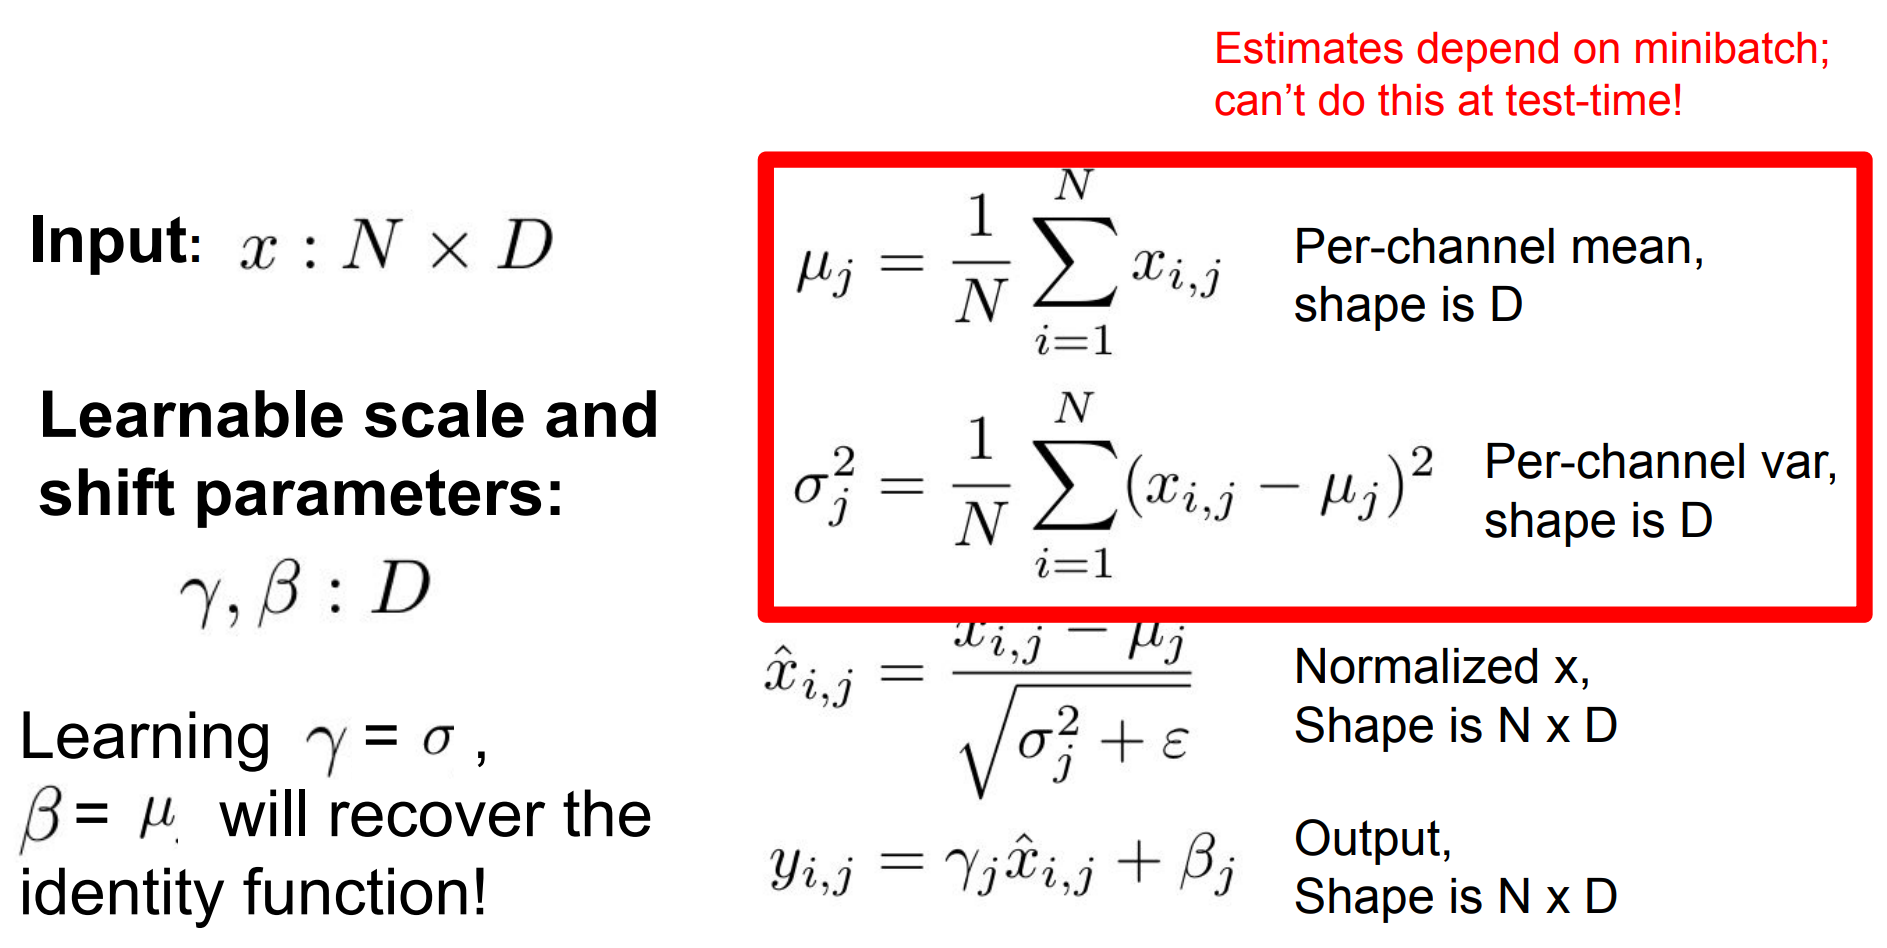
\includegraphics[width=1.0\textwidth,height=0.9\textheight,keepaspectratio]{./images/batch_norm_2.png}
% \end{figure}
% \end{frame}

% \begin{frame}{Batch Normalization}
% \begin{figure}
% \centering
% 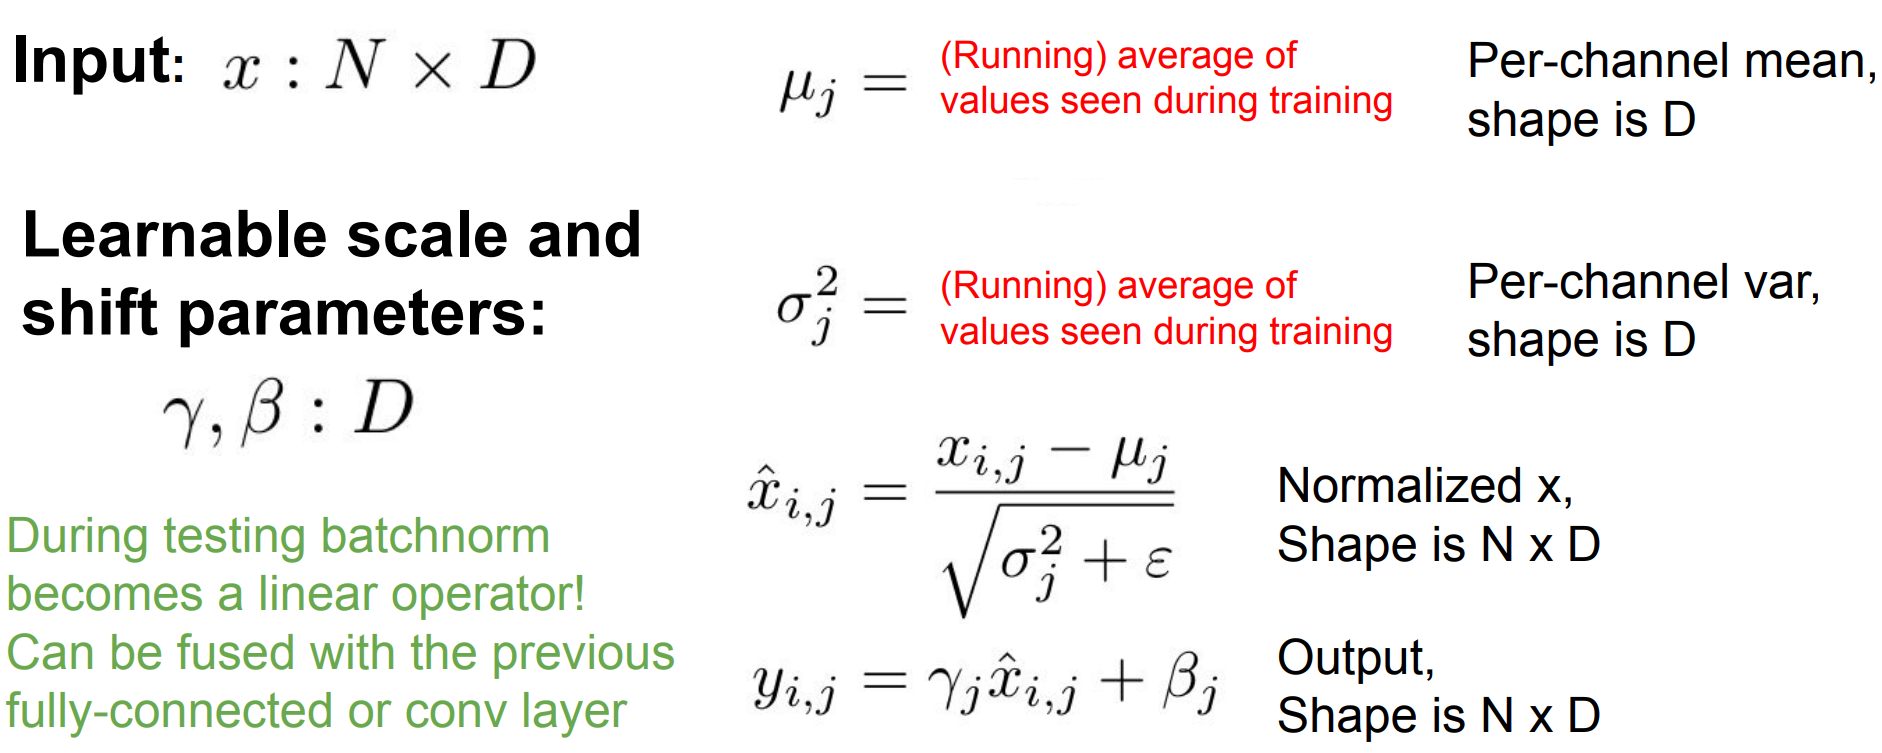
\includegraphics[width=1.0\textwidth,height=0.9\textheight,keepaspectratio]{./images/batch_norm_3.png}
% \end{figure}
% \footnotetext{Slide based on CS231n by Fei-Fei Li, Yunzhu Li \& Ruohan Gao}
% \end{frame}

% \begin{frame}{Batch Normalization}
% \begin{figure}
% \centering
% 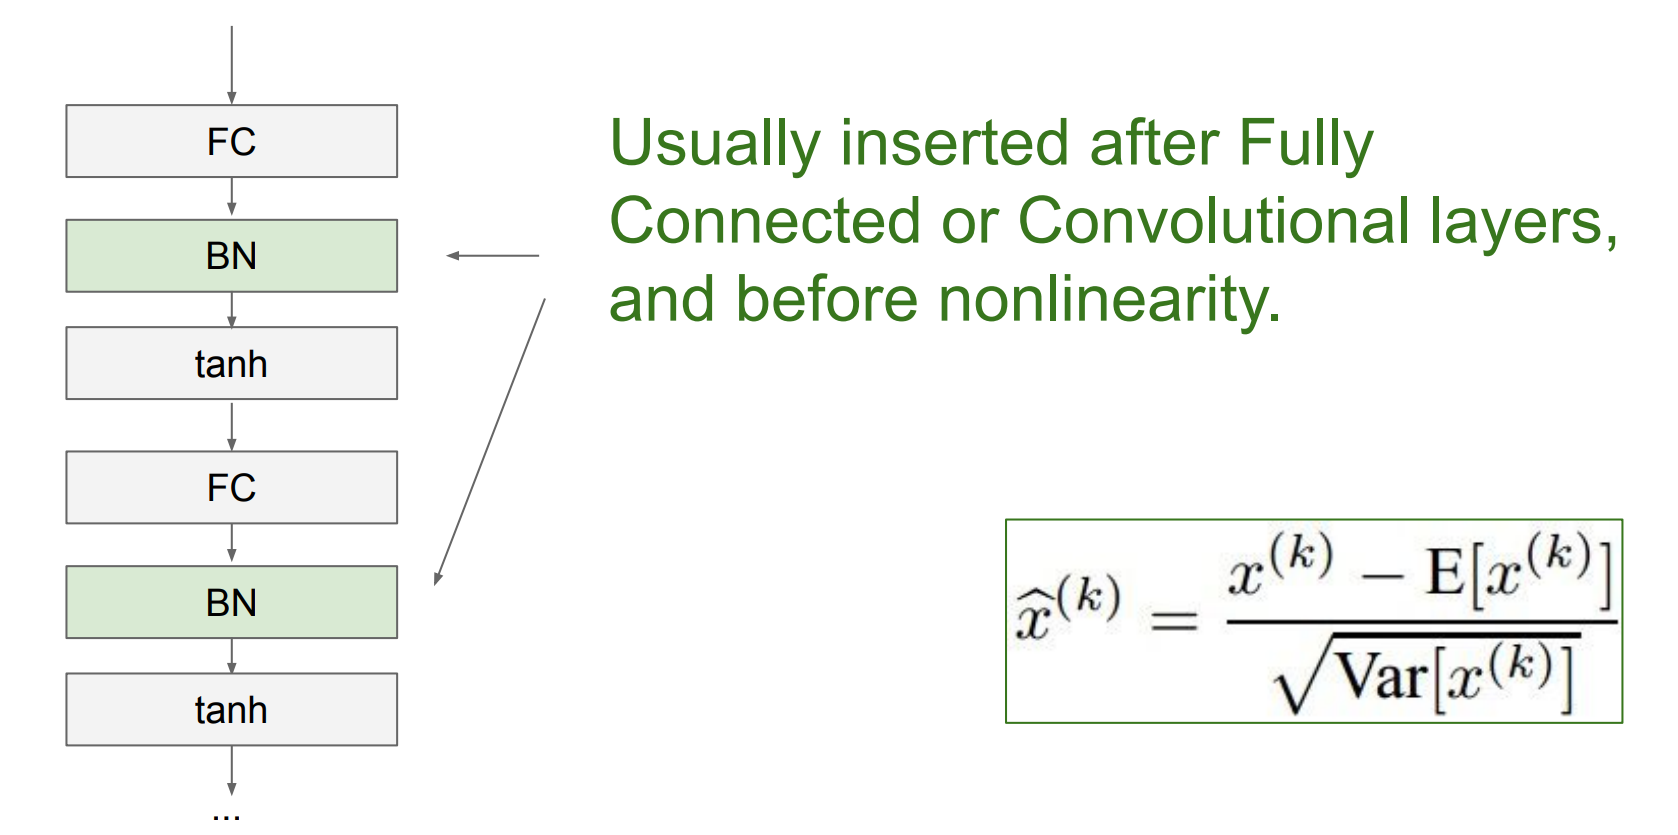
\includegraphics[width=1.0\textwidth,height=0.9\textheight,keepaspectratio]{./images/batch_norm_4.png}
% \end{figure}
% \end{frame}

% \begin{frame}{Batch Normalization}
% \begin{figure}
% \centering
% 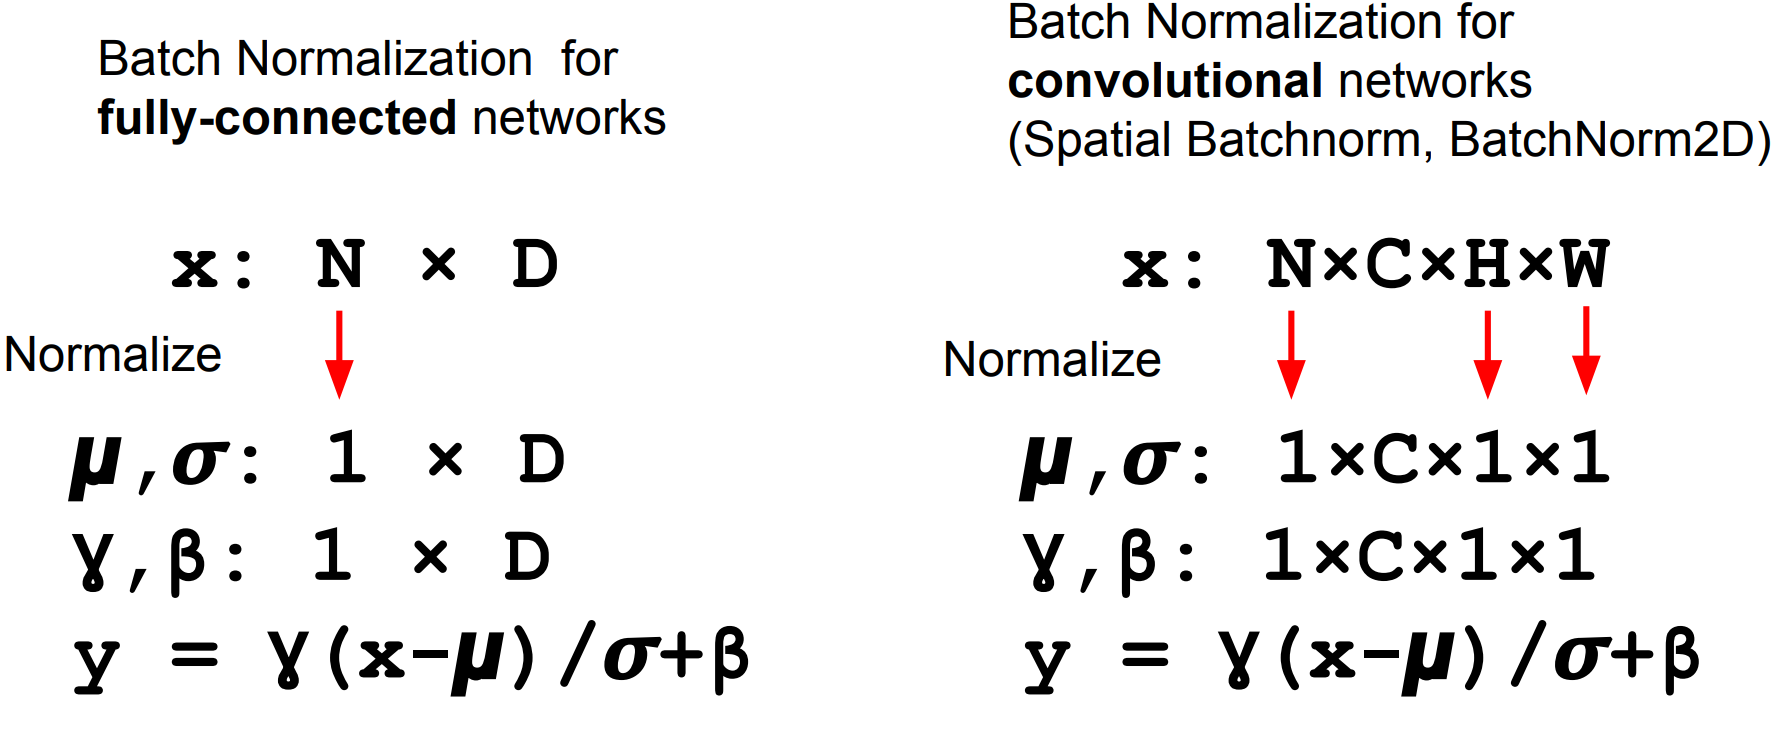
\includegraphics[width=1.0\textwidth,height=0.9\textheight,keepaspectratio]{./images/batch_norm_5.png}
% \end{figure}
% \footnotetext{Slide based on CS231n by Fei-Fei Li, Yunzhu Li \& Ruohan Gao}
% \end{frame}

\begin{frame}{Batch Normalization}
\begin{itemize}
    \item Advantages:
    \begin{itemize}
        \item Makes deep networks much easier to train!
        \item Improves gradient flow
        \item Allows higher learning rates, faster convergence
        \item Networks become more robust to initialization
        \item Acts as regularization during training
        \item Zero overhead at test-time: can be fused with conv!
    \end{itemize}
    \pause
    \item Disadvantages:
    \begin{itemize}
        \item Behaves differently during training and testing: this is a very common source of bugs!
    \end{itemize}
\end{itemize}
\footnotetext{Slide based on CS231n by Fei-Fei Li, Yunzhu Li \& Ruohan Gao}
\end{frame}

\begin{frame}{Batch Normalization}
\begin{figure}
\centering
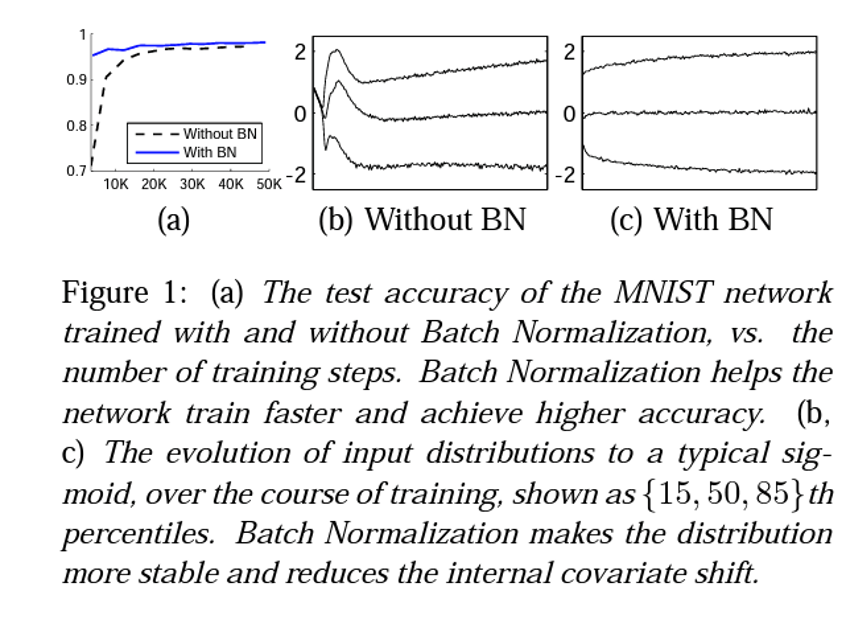
\includegraphics[width=1.0\textwidth,height=0.9\textheight,keepaspectratio]{./images/batch_norm_6.png}
\end{figure}
\footnotetext{\href{https://arxiv.org/pdf/1502.03167v3.pdf}{Ioffe and Szegedy 2015}}
\end{frame}

% \begin{frame}{Things to Remember}
%     \begin{itemize}
%         \item Training Deep Networks
%         \begin{itemize}
%             \item Dropout
%             \item Data augmentation
%             \item Activation
%             \item Batch normalization
%         \end{itemize}
%         \item Transfer learning
%         \begin{itemize}
%             \item Always use Fine-tuning when possible
%         \end{itemize}
%     \end{itemize}

% \end{frame}

% \begin{frame}{Full Deep Learning Pipeline}
% \begin{itemize}
%     \item Data Pre-processing
%     \item Architecture
%     \item Loss
%     \item Optimizer
%     \item DataLoaders
%     \item Data Augmentation
%     \item Fine-Tuning
%     \item Ensembling
% \end{itemize}
    
% \end{frame}



\begin{frame}{Full Training Workflow}
\begin{itemize}
    \item \textbf{Step 1: Initial Setup}
    \begin{itemize}
        \item Start with a pretrained model and just finetune when possible; it saves time and improves results.
        \item Define an initial architecture without regularization (e.g., dropout) or augmentations.
        \item Set up validation strategy and choose an appropriate evaluation loss and metric.
        \item Train the model to get a \textbf{baseline score}.
    \end{itemize}
    
\end{itemize}
\end{frame}

\begin{frame}{Full Training Workflow}
\begin{itemize}
    \item \textbf{Step 2: Improvement Process}
    \begin{itemize}
        \item Overfitting is common at the start; use regularization techniques like:
        \begin{itemize}
            \item Dropout, batch normalization,...
        \end{itemize}
        \item Perform error analysis to identify weaknesses and choose appropriate augmentations or preprocessing.
        \item Tune hyperparameters: layers, epochs, learning rate, batch size, etc.
        \item Optionally, use ensembling to boost scores (requires more resources).
    \end{itemize}
    \item \textbf{Key Tip:} Track scores and improvements at every step to measure progress effectively.
\end{itemize}
\end{frame}


\begin{frame}{Full Training Workflow}
\begin{itemize}
    
    \item \textbf{Step 3: Finalization}
    \begin{itemize}
        \item Save the optimized model for deployment.
        \item Use the model for inference in real-world applications.
    \end{itemize}
    
\end{itemize}
\end{frame}


\end{document}